\documentclass[12pt]{article}
%\renewcommand{\baselinestretch}{1.15}
\usepackage{natbib,amsmath,amsthm,booktabs,subfigure,anysize,hyperref,graphicx,float,bbm,epstopdf}
\usepackage[margin=1in]{geometry}
\bibliographystyle{aea}
%\bibliographystyle{apalike}
%\bibliographystyle{aernobold}
%\bibliographystyle{economet}
%\marginsize{2cm}{2cm}{2cm}{2cm}

\usepackage{threeparttable}
\usepackage{array} % for adding extra space between table columns
\usepackage{booktabs} % for adding extra space between table columns
\usepackage{multirow}
\usepackage{xcolor}
\usepackage{bm}
\definecolor{dark-red}{rgb}{0.4,0.15,0.15}
\definecolor{dark-blue}{rgb}{0.15,0.15,0.4}
\definecolor{medium-blue}{rgb}{0,0,0.5}
\definecolor{ChadBlue}{rgb}{.1,.1,.5}
% Chad's colors:
% See http://web.njit.edu/~kevin/rgb.txt.html for possibilities
\definecolor{ChadDarkBlue}{rgb}{.1,0,.1}
\definecolor{ChadBlue}{rgb}{.1,.1,.5}
\definecolor{ChadRoyal}{rgb}{.2,.2,.8}
%\definecolor{ChadGreen}{rgb}{0,.35,.1}
%\definecolor{ChadGreen}{rgb}{0,.5,.25}  % Too bright
%\definecolor{ChadGreen}{rgb}{0,.4,.2}    % Still too bright
\definecolor{ChadGreen}{rgb}{0,.4,0}    % Dark Green
%\definecolor{ChadRed}{rgb}{.8,.1,.2}    % Too bright
\definecolor{ChadRed}{rgb}{.5,0,.5}  % purple
\hypersetup{
    colorlinks, linkcolor=ChadRed,
    citecolor=ChadBlue, urlcolor=ChadBlue
}
\newcommand\posscite[1]{\citeauthor{#1}'s (\citeyear{#1})}
\setlength{\parskip}{0.15cm}
\newtheorem{proposition}{\color{ChadGreen} Proposition}
\newtheorem{finding}{\color{ChadGreen} Finding}
\newtheorem{SF}{\color{ChadGreen} Stylized fact}
\newtheorem{hyp}{Hypothesis}
\newtheorem{fact}{Fact}
\newtheorem{prop}{Proposition}
\usepackage{caption}
%\usepackage[font=small,labelfont={color=ChadBlue,bf}]{caption}
\usepackage[font=small,labelfont=bf]{caption}
%\usepackage{subcaption}
%\usepackage{subfloat}
\usepackage{amssymb}
\usepackage{amsfonts}
\usepackage{amsmath}
\usepackage{accents}
\usepackage{color,soul}
\usepackage{smartdiagram}
\usepackage[figuresright]{rotating} % Rotating table
\usepackage{lscape} % Rotating table
\usepackage{diagbox}
\usepackage{multicol}
\usepackage{tikz}
\usepackage{comment}
\usepackage{float}

\newcommand{\ubar}[1]{\underaccent{\bar}{#1}}
\usepackage{setspace}  %using this package conflicts with footnote hyperlink jump. Using this package makes the footnote links inactive.
\usepackage[all]{hypcap}        % needed to help hyperlinks direct correctly;
%\renewcommand{\sfdefault}{ptm}

\newtheorem{theorem}{Theorem}
\newtheorem{cor}[theorem]{Corollary}
\renewcommand{\proof}{\noindent \textbf{Proof.\ }}
\newtheorem{conjecture}{Conjecture}
\newtheorem{example}{Example}
\newtheorem{defn}{Definition}
\renewcommand{\qed}{\hfill\rule{2.1mm}{2.1mm}}
%\newtheorem{proposition}{\color{ChadGreen} Proposition}
%\newtheorem{finding}{\color{ChadGreen} Finding}
%\newtheorem{SF}{\color{ChadGreen} Stylized fact}
% Fix title, sections, etc.
\newcommand\fnote[1]{\captionsetup{font=small}\caption*{#1}}

\let\LaTeXtitle\title
%\renewcommand{\title}[1]{\LaTeXtitle{\color{ChadBlue}{\LARGE #1}}}
%\renewcommand{\abstractname}{\color{ChadBlue}Abstract}
%\renewcommand{\figurename}{\color{ChadBlue}Figure}
%\renewcommand{\tablename}{\color{ChadBlue}Table}
\renewcommand{\arraystretch}{1.1} % space between rows

\usepackage{sectsty}
%\allsectionsfont{\color{blue}\itshape\underline}
%\sectionfont{\color{ChadBlue}}
%\subsectionfont{\color{ChadBlue}}
%\subsubsectionfont{\color{ChadBlue}}
\usepackage{lscape}
\graphicspath{{figure/}}
\newcolumntype{P}[1]{>{\centering\arraybackslash}p{#1}}

%\newcommand\YUGE{\fontsize{30}{40}\selectfont}

\linespread{1.2}
\geometry{a4paper,scale=0.75}
\setlength{\parskip}{0.5em}

%---------------------------------------------------------------------------------------

\begin{document}

\title{  \Large \textbf{Exchange Rate Pass-Through and Importers' Credit Constraints: Evidence from China} 
\thanks{We thank David Edward Cook, Juanyi Jenny Xu, Edwin L.-C. Lai, Dmitry Mukhin, and all participants of HKUST Center of Economic Policy Brownbag Seminar (2023) and HKUST Macroworkshop (2022) for helpful comments. All errors are those of the authors.}}

\author{\large \href{http://yaoli.people.ust.hk/}{Yao Amber Li}\thanks{Li: Department of Economics and Faculty Associate of the Institute for Emerging Market Studies (IEMS), Hong Kong University of Science and Technology, Clear Water Bay, Kowloon, Hong Kong SAR-PRC. Email: \href{mailto:yaoli@ust.hk}{yaoli@ust.hk}.}\\ \large{HKUST}
\and \large \href{}{Lingfei Lu}\thanks{Lu: Department of Economics, Hong Kong University of Science and Technology, Clear Water Bay, Kowloon, Hong Kong SAR-PRC. Email: \href{mailto:}{lingfei.lu@connect.ust.hk}.} \\ \large{HKUST}
 }

\date{\today }

\maketitle

\begin{abstract}
Exchange rate fluctuation is a key factor that affects international trade prices. This paper studies the exchange rate pass-through patterns in China and its linkage with importers' credit constraints. Using Chinese firm-level information and customs transaction records from 2000 to 2007, we find that (1) the average level of exchange price pass-through into import prices in China is about 2/3, far below the nearly complete export price pass-through; (2) for importers in financially more constrained industries, exchange rate pass-through tends to be more complete; (3) a higher degree of import source diversity can effectively lead to a less complete pass-through and offset the effects of credit constraints. This suggests that a more diverse sourcing network can enhance the bargaining power of buyers and alleviate the impact of financial imperfections on trade.

\end{abstract}

\textbf{Keywords:} Exchange rate pass-through, Exchange rate disconnect, Credit constraints, Import prices, Market power, China.

\textbf{JEL Codes:} F14, F31, F41.

\section{Introduction} \label{Introduction}

Why do exchange rate fluctuations not result in price changes of the same magnitude? This is one of the core questions among a set of ``exchange rate disconnect'' puzzles (\cite{obstfeld2000}). As price signals in the international trade market, exchange rates appear less informative to firms than expected. Exchange rate pass-through (ERPT) defined as the elasticity of local price changes to exchange rate fluctuations, varies widely across countries, industries, and time. Existing studies have generated widely varying estimates of the exchange rate pass-through. It is particularly attractive for researchers in international trade and open macroeconomics to demystify the ``exchange rate disconnect" puzzles. Understanding the pattern of exchange rate pass-through has important implications for formulating macro policy, including monetary policy, inflation targeting, and the balance of payments.

In this paper, we focus on the role of importers in determining exchange rate pass-through and connect it with firms' financial constraints. This article tends to fill a gap in the literature by linking market power on both sides of international trade. We provide a novel perspective to study the nature of exchange rate disconnect for emerging markets, where firms are more vulnerable to credit constraints due to immature financial markets. In contrast to the conventional framework of exchange rate pass-through, where importers are mostly price takers, we contribute to the literature by identifying the importers' implicit sourcing power and comparing their heterogeneous capacity to absorb exchange rate shocks. We will compare firm-level exchange rate pass-through into import and export prices to reflect the similarities and differences between the market power of Chinese firms in both markets. Going further, if a country's import and export exchange rate pass-through patterns differ significantly, this may even affect terms of trade and current account imbalances. We believe that micro-evidence from import exchange rate pass-through provides a new perspective to study the ``exchange rate disconnect" puzzle.

Using Chinese micro-level data, we estimate the exchange rate pass-through as the price elasticity of import prices concerning real exchange rates. Specifically, we merged the annual surveys of Chinese Industrial Enterprises with the transaction records from China’s customs. We adopted fixed effects panel regressions with first-order differences to capture the changes in product prices and real exchange rates. The average estimated exchange rate pass-through into import prices in China during 2000-2007 is around 70\%, which is obviously less complete compared to the over 95\% pass-through into export prices. Second, we identify the effects of credit constraints on importers' exchange rate pass-through. We use US measures of sectors’ financial constraints (\cite{manova-wei-zhang2015}) in our main empirical analysis while using Chinese measures of credit needs (\cite{fan-li-yeaple2015}) for robustness checks. In our baseline results, import prices for firms in sectors with higher financial constraints are more sensitive to exchange rate shocks. Third, we calculate the proxy for an importer's sources (countries) and find that an importer with more alternative supplier options can resist the effects of credit constraints and absorb exchange rate shocks better.

To support our empirical analysis, we conduct six groups of robustness check tests. First, we compare sector-level credit constraint variables calculated from China and US data as alternative measures. Second, we exclude countries that use the US dollar as their fiat currency or adapt the USD-pegged exchange rate regime. Third, we divide observed firms into two-way traders (simultaneous import and export in the same year) and pure importers (only import in a certain year). We check our results using only the two-way traders who account for the vast majority of trading firms and trade volume. Fourth, we further control firm ownership types: domestic private firms, state-owned firms, and multinational firms. Fifth, we estimate the firm-level markup following \cite{dlw2012} and test whether markups affect our main results. Finally, we utilize alternative estimation methods, such as alternative fixed effects and cross-sectional specifications. These results are all significant and robust. In the discussion, we confirm that firms with different market shares also demonstrate heterogeneous price responses to exchange rate changes. Although firm heterogeneity in those aspects affects exchange rate pass-through, credit constraints still play an unignorable role even after we control those firm characteristics. 

We show that importers' credit constraints influence price-setting patterns in international trade. We provide evidence for three key findings: (1) the average import exchange rate pass-through level in China is significantly less complete than the export one; (2) importers' financial constraints will increase exchange rate pass-through into both prices to be more complete; and (3) importers who import a certain product from more sources (higher source diversity) have a less complete pass-through. In other words, financially constrained importers will absorb more price fluctuations caused by exchange rate changes, and financially constrained exporters will pass through more exchange rate changes to prices than unconstrained firms. This reflects that binding financial constraints will lead to limited buyers' sourcing market power for importers and narrow pricing-to-market margins for the sellers. Importers with a wider sourcing base could get more access to alternative options and avoid bargaining disadvantages in exchange rate fluctuations to some extent.

This paper contributes to three strands of literature. First, this article contributes to a large literature on exchange rate disconnect (\cite{obstfeld2000}), particularly on the response of trade pricing to exchange rate changes (\cite{campa2005}). Trade prices denominated in the destination currency are usually much less volatile than exchange rates. Recently, more studies have linked exchange rate pass-through to disaggregated firm-level characteristics. \cite{bmm2012} find that exporters with better performance react to exchange rate shocks by adjusting their markup more and less their export volume. \cite{aik2014} find that firms with higher import intensity and greater market share have less complete price pass-through. Many follow-up works find that exporters' productivity (\cite{lmx2015}) and product quality (\cite{chen2016}; \cite{auer2018}), as well as their imported inputs (\cite{wang-yu2021}), market shares (\cite{auer2016}; \cite{devereux2017}) and information access (\cite{garetto2016}), will all affect the export exchange rate pass-through. \cite{lmx2015} find nearly complete exchange rate pass-through into local prices for Chinese exporters, which means that their response to the price of their domestic currency (RMB) is very weak. However, the role of importers in determining exchange rate pass-through remains a novel field to study (\cite{alviarez2023}). Our contribution is to provide micro-level evidence of importers' heterogeneity in response to exchange rate shocks when firms operate in industries with different degrees of credit constraints. This supports the idea that the characteristics of both importers and exporters influence international trade pricing. We believe that the bargaining power of importers, an important yet underexplored force determining pricing patterns in the global market, may help explain the puzzle of the ``exchange rate disconnect''. 

Second, we contribute to the literature on how credit constraints affect the price-exchange rate elasticity. We study the influence of sector-level credit constraints on the response of import prices to exchange rate fluctuations. The most relevant study for this paper is \cite{strasser2013}, which discusses the relationship between exchange rate pass-through and exporters' credit conditions. \cite{strasser2013} uses a firm-level survey to show that financially constrained exporters pass exchange rate shocks to prices more completely. Subject to variable markups, firms under borrowing constraints must keep the pricing-to-market (PTM) strategy to a limited extent because they have less space to adjust their profit margin. \cite{dai2021} finds that exchange rate pass-through to export prices denominated in home currency is lower for firms under tighter financial constraints. However, they focus on aggregate firm-level export behaviors while we assess bilateral trade elasticity with each country instead. Our paper differs from earlier studies in that: first, we focus on importers whose pricing behaviors are also affected by credit constraints; second, with the detailed Chinese panel data, we could estimate the relationship between credit constraints and price response to exchange rate shocks at the firm-source-product-year level, controlling for various variables and their interactions.

Third, this paper relates to the broader literature on credit constraints and international trade. Cross-border logistics is riskier than domestic sales or purchasing, and contractual reliability in international transactions is weaker. Therefore, it is widely believed that trade participants rely on additional external capital to pay fixed costs to source or export to other countries, which cannot be fully covered by internal cash flows from operations (\cite{manova2013}, \cite{chaney2016}). \cite{feenstra-li-yu2014}, \cite{manova-wei-zhang2015}, \cite{fan-lai-li2015} provide comprehensive theoretical explanations and empirical evidence from China about how credit constraints affect exports through incomplete information, multinational links, and quality, respectively. Recently, \cite{xu-guo2021} demonstrated that the estimated exchange rate elasticity of export volume negatively correlates with the sector’s financial constraints. However, controlling markup adjustment could not entirely eliminate the financial constraints' effect, leaving room for further research. In the context of exchange rate shocks, our study deliberately examines how credit constraints affect importers' sourcing behavior. This provides a novel perspective to study the exchange rate disconnect puzzle in emerging markets, where firms are usually financially more vulnerable due to immature financial markets.

The remainder of this paper is organized as follows. Section \ref{Data&Measurements} describes the data and measurements of the key variables. Section \ref{Empirical} introduces our empirical identification strategies and the main results on credit constraints and exchange rate pass-through. Section \ref{Robustness} examines the robustness of our results.  Section \ref{Discussion} further discusses how buyer-side sourcing power affects exchange rate pass-through. In Section \ref{Conclusion} we provide concluding comments.

\section{Data and Measurements} \label{Data&Measurements}

Our empirical analysis relies on a comprehensive micro-database of Chinese importers and exporters and macro-level indicators. This section describes these data and measurements of key variables from various sources and also presents summary statistics of those samples.

\subsection{Data} \label{Data}

We conduct our empirical tests using various data sources: (1) country-level exchange rates and other macro data from the Penn World Table (PWT) 10.0 and the International Financial Statistics (IFS); (2) the Chinese Customs Database from China’s General Administration of Customs; (3) the Annual Survey of Industrial Enterprise (ASIE) from National Bureau of Statistics of China for firm-level accounting information from the National Bureau of Statistics of China (NBSC). This section will introduce the basic information about these datasets and a brief description of the sample construction process.

\subsubsection{Country-level macro data} \label{Data-Macro}

We obtain annual bilateral nominal exchange rates from the Penn World Table (PWT) 10.0 referring to \cite{feenstra2015}, and consumer price indices (CPI) from the International Financial Statistics. We keep all countries that keep full records of exchange rates and CPI from 1999 to 2011 and trade with China, resulting in 154 countries and regions. Those major trading partners account for more than 95\% of the Chinese total import and export value every year.

Following the convention, the bilateral nominal exchange rate ($NER_{ct}$) is defined as the number of home currency units that can purchase a unit of foreign currency. By this definition, an increase in $NER_{ct}$ means a nominal depreciation of the Chinese RMB against this currency from country $c$ in year $t$. Following \cite{lmx2015}, the CPI-based real exchange rate ($RER_{ct}$) is defined as the nominal exchange rate multiplied by the foreign consumer price index and divided by the Chinese consumer price index at the same year, which is

$$
RER_{ct}=NER_{ct} \cdot \frac{CPI_{ct}}{CPI_{CHN,t}}.
$$

Similarly, an increase in $RER_{ct}$ means a real depreciation of the Chinese RMB against the foreign country $c$'s currency. In later specifications, we mainly use the first difference of the logarithm of the real exchange rate to represent exchange rate changes.

Changes in nominal and real exchange rates for the U.S. dollar and the euro relative to Chinese RMB (level in 1999 as base value 100) are shown in figures \ref{fig.ER} We could observe that the real exchange rates against the US dollar were relatively stable in 2000-2004 due to the nominal pegging scheme of RMB to USD. In July 2005, the peg was lifted to a slight appreciation of RMB against US dollars due to this exchange policy evolution. However, the exchange rates of the Chinese RMB against the Euro (and other floating currencies) fluctuated up and down during the whole period. 

\begin{figure}[htbp]
	\centering
	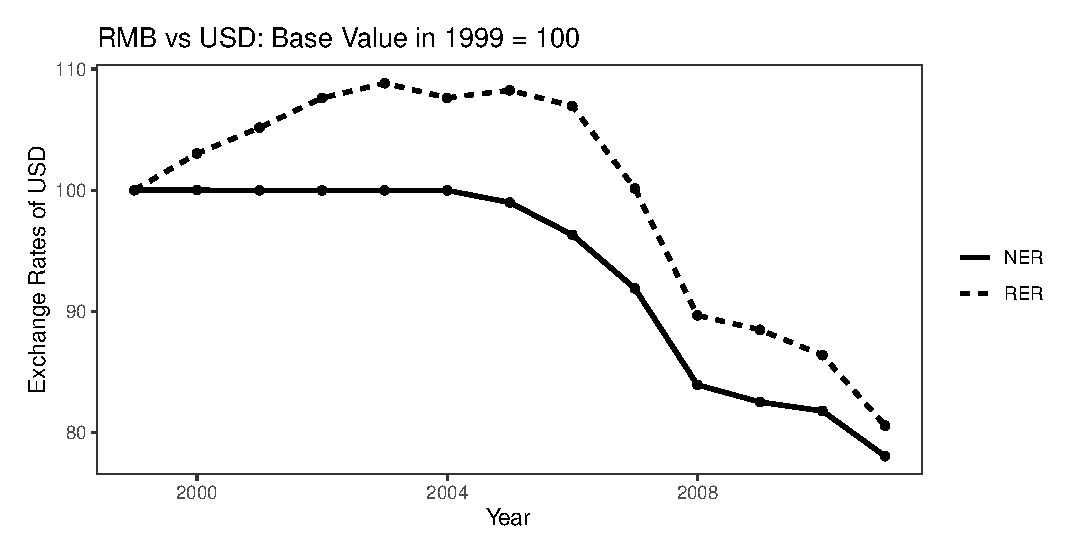
\includegraphics[width=1\textwidth]{R/USD.eps}
	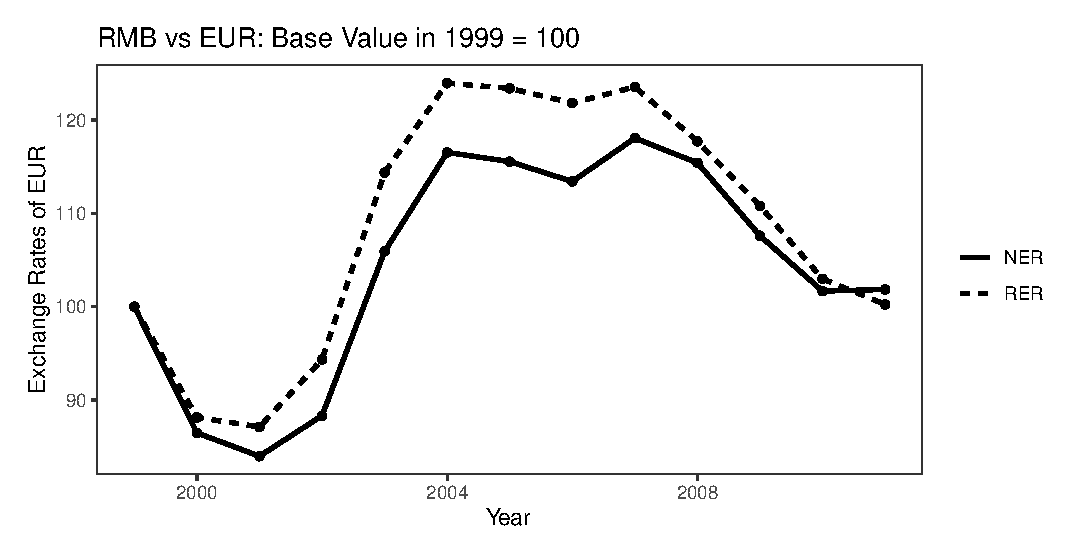
\includegraphics[width=1\textwidth]{R/EUR.eps}
	\caption{Exchange rates of Chinese RMB against USD and euro (1999-2011)}
	\label{fig.ER}
\end{figure}

In addition to nominal and real exchange rates, we use the real GDP of foreign countries of PWT 10.0. Real GDP is calculated with growth rates from the national account. The controls of real GDP changes of the destination country, $\Delta RGDP_{ct}$, help us exclude the effect of aggregate economic growth and market demand on price movements. All macro variables, including exchange rates and real GDPs, are in annual terms to match the customs record with the firm information.

\subsubsection{Customs transaction-level data} \label{Data-Customs}

For trade details, we use the transaction-level records from the General Administration of Customs of China (GACC). The whole sample period ranges from 2000 to 2011. This dataset includes the most comprehensive information on all Chinese trade transactions, including each firm's import or export value (denominated in US dollars), quantity, unit, product name and code, source or destination country, and the type of enterprises (e.g., state-owned, private, foreign-invested, and joint ventures), etc. Using these detailed trade records, we can compute firm–product unit values to proxy the export and import prices.

We separate the complete records into export and import parts. In our analysis, each unique transaction refers to a firm-product-country-year pair. The categories of products in China's customs trade records are coded according to the Harmonized Coding and Description System (HS) of the World Customs Organization (WCO). The original data are subject to HS 8-digit classification. Since there were two major revisions of the HS system in 2002 and 2007, we aggregate HS8 product-level information to the HS6 level and then use conversion tables from the United Nations Trade Statistics to convert HS 2007 and 2002 codes into the older version of HS 1996 as in \cite{fan-li-yeaple2015}.

For later empirical studies, we drop unwanted observations referring to the standard of \cite{lmx2015}: (1) products with inconsistent missing information of unit or quantity; (2) special product categories such as arms (HS2=93), antiques (HS2=97), and special categories (HS2=98 and 99); (3) transactions existing for only one year without any change over time. These outliers make up only a tiny part of the observations. We will refer to this data set as the ``whole sample'' in the subsequent analysis.

\subsubsection{Chinese firm-level data} \label{Data-CIE}

Our source of Chinese firm-level production and financial information is the Annual Surveys of Industrial Enterprises in China (ASIE) conducted by the National Bureau of Statistics of China (NBSC). This database includes all state-owned enterprises and above-scale firms with more than 5 million RMB in annual sales. The dataset covers the period from 1999 to 2007. The number of firms each year ranged from about 130,000 in 1999 to 300,000 in 2007. The data provide details about firms’ identification codes, ownership, industry type, and about 80 other accounting variables in the balance sheet. The company information variables in this project include each firm's number of employees, total wage payment, fixed asset value, sales income, total operation inputs, etc. We also use firms’ registration types to categorize them as state-owned enterprises (SOEs), domestic private enterprises (DPEs), multinational firms (MNEs), and joint ventures (JVs).

To merge these firm-level survey data with customs records, we follow the standard procedure to match the identification codes based on the contact information of the firms as in \cite{fan-li-yeaple2015}. Manufacturing firms participating in international trade in the matched sample are uniquely identified by each observation's FRDM (legal entity) code and the survey year. We drop unsatisfactory observations referring to the criteria of \cite{bkl2021}.\footnote{We drop firms with less than ten employees and firms with incomplete information or discrepancies (e.g., negative sales or input usage). Ignoring these micro-level firms has no significant impact on our study of the pricing patterns of Chinese importing firms.} This merged sample contains the overlapping time of the two datasets, i.e., from 2000 to 2007, and all indicators are in annual terms. We will refer to this combined dataset as the ``matched sample" in the rest of this paper.

The summary statistics of the entire customs records, the firm information dataset, and the final matched sample are shown in panels A, B, and C in Table \ref{tab.summary.sample}, respectively. The notable point is that for all variables involved in the amount of money in the table, the mean value is much larger than the median and the mean of some variables is even larger than its 90\% quantile. This implies that the distribution of trade value is very uneven and close to the right long tail shape., with a few large transactions accounting for the majority of trade value.

\begin{table}[htbp]
        \centering
	\caption{Summary statistics for customs and firm data}
	\label{tab.summary.sample}
	\resizebox{\textwidth}{!}{
	\begin{threeparttable}
	\begin{tabular}{lcccccc}
		\toprule
            & \multicolumn{1}{l}{\#observations} & \multicolumn{1}{l}{Mean} & \multicolumn{1}{l}{Median} & \multicolumn{1}{l}{Std. dev} & \multicolumn{1}{l}{P10} & \multicolumn{1}{l}{P90} \\
		\textbf{Panel A: Customs records} &       &       &       &       &       &  \\
		Export Price (RMB/unit) & 18,581,221 & 22007.45 & 30.1042 & 2229173 & 4.5645 & 556.4724 \\
		Annual Export Price Change & 11,400,795 & 0.0259 & 0.0060 & 0.6653 & -0.5001 & 0.5709 \\
		Import Price (RMB/unit) & 14,172,315 & 49519.78 & 111.0406 & 1411944 & 5.1594 & 10247.12 \\
		Annual Import Price Change  & 8,580,234 & 0.0236 & -0.0021 & 1.0171 & -0.8523 & 0.9388 \\
		\midrule
		\textbf{Panel B: Firm information} &       &       &       &       &       &  \\
		Sales Income (×1000 RMB) & 1,745,511 & 78826.33 & 17630 & 714350.5 & 5318  & 111319 \\
		Employment (persons)& 1,745,511 & 262.95 & 108   & 964.64 & 30    & 500 \\
		Fixed Asset (×1000 RMB) & 1,745,511 & 27437.2 & 4043  & 312024.8 & 573   & 36968 \\
		Operation Input (×1000 RMB) & 1,745,511 & 61682.99 & 13971 & 562923.1 & 4035  & 168810 \\
		Current wage payable (×1000 RMB) & 1,745,511 & 3730.16 & 1121  & 28699.16 & 266   & 6300 \\
		\midrule
		\textbf{Panel C: Matched sample} &       &       &       &       &       &  \\
		Export Price (RMB/unit) & 1,724,591 & 15960.54 & 28.7442 & 1806021 &  5.1482 & 380.3671 \\
		Annual Export Price Change & 1,724,591 & 0.0248 & 0.0056 & 0.7101 & -0.5251 & 0.5940 \\
		Import Price (RMB/unit) & 1,478,176 & 23573.29 & 81.9251 & 447447 & 4.9166 & 4169.39 \\
		Annual Import Price Change  & 1,478,176 & -0.0851 & -0.0018 & 1.4129 & -1.3406 &  1.1411 \\
		\bottomrule
	\end{tabular}
	\begin{tablenotes}
		\footnotesize
		\item[Notes:] This table shows the summary statistics of some important variables in our three major datasets. Panel A and panel C describe the total annual average prices and price changes for the whole and matched samples, respectively. The observations in panel A and panel C are at the firm-product-country-year level. The price in panel A and panel C are in RMB. Panel B describes sales and costs information of Chinese manufacturing firms during 2000-2007. The money values in panel B are in thousands of RMB. The observations in panel B are at the firm-year level.
	\end{tablenotes}
	\end{threeparttable}
        }
\end{table}

\subsection{Measurements of credit constraints} \label{Measurements-Credit Constraints}

A critical issue in our empirical strategy is to measure the extent of financial constraints. In this article, we use several proxy methods for sector-level financial vulnerability to measure the credit constraints faced by Chinese importers following \cite{manova2013}. To deal with potential concurrent endogeneity, our measures of credit constraints are applied to each firm throughout the period. Following a widely recognized literature on the role of credit constraints in international trade (\cite{kroszner2007}; \cite{manova2013}; \cite{manova-wei-zhang2015}; \cite{fan-lai-li2015}), we use multiple financial constraint measures at the sector level to proxy for credit needs (demand for outside capital) and ability to resist financial risks. These measures are designed to reflect the nature of each industry, which should be regarded as exogenous for each firm. A firm in a more financially vulnerable industry tends to face a tighter credit constraint, regardless of its current operating conditions.

The first measure we use is external finance dependence ($ExtFin_j$), defined as the share of capital expenditures not financed by operational cash flows. If external finance dependence is high, the industry is more financially vulnerable, and firms in this industry are more credit-constrained. The second measure is asset tangibility ($Tang_j$), which describes the share of the net value of tangible assets that firms can pledge as collateral to raise external finance to its total book value. The third measure is the inventory-to-sales ratio ($Invent_j$), which measures the production cycle duration and the necessary working capital to maintain inventories and meet demand. 

To utilize the U.S. industry-level credit measures in the literature, we match China's CIC industry code system to the International Standard Industrial Classification (ISIC) system. We first convert 3- and 4-digit industries in the older ISIC Revision 2 from \cite{manova-wei-zhang2015} to match the newest ISIC Revision 3 codes; then we link the ISIC Revision 3 codes to the adjusted CIC codes in the CIE datasets. Finally, we match the firms in the merged sample to those sector-level financial constraint measures. For those many-to-one scenarios, when matching industry types, we assign the average value from source industries to the master industry. In this way, each Chinese firm in our sample is assigned a unique value for each credit measure.

Although we construct three measures of credit constraints as in the literature, we will mainly focus on external finance dependence and tangibility in our later analysis. One important reason is that their interpretation can be linked to firms' exposure and resistance to financial frictions directly. On the contrary, the inventory ratio may be related to inventory management efficiency rather than liquidity and financial reasons. Following \cite{manova-wei-zhang2015}, we also construct the first principal component of external finance dependence and asset tangibility $FPC_j$, which increases with the former and decreases with the latter. An industry with a higher $FPC_j$ is more financially sensitive in which firms require more outside funds but own less collateralizable assets. Therefore, we could use $FPC_j$ as an aggregate measure of financial constraints that combines information from external finance dependence and asset tangibility.

We have two reasons for using credit constraint measures based on US data in our main regressions. First, we want to remove the distortion caused by the limited credit supply in China and focus on the credit demand associated with sector-level characteristics. A nice feature of using US data to calculate credit constraint measures is that, because the US has a financially developed credit market, there is no concern that credit shortages may distort the estimation of true credit demand in an industry. Second, the U.S. patterns of sector-level credit demand are proved persistent in a cross-country setting in the literature (\cite{kroszner2007}; \cite{manova-wei-zhang2015}; \cite{fan-lai-li2015}), especially when the industry classification is broadly defined. Intuitively, the financial needs of an industry can differ in levels across countries. Still, the relative ranking between industries is supposed to be determined only by technical reasons specific to the industry itself.

Alternatively, we compute all credit measures, external finance dependence ($ExtFin_j$), asset tangibility ($Tang_j$), and inventory ratio ($Invent_j$) based on Chinese firm-level information from ASIE. First, we adopt the estimated value of external finance dependence from \cite{fan-lai-li2015}. Then we calculate the inventory ratio as the value of inventory over sales income, the asset tangibility as the value of fixed assets over total assets, and the R\&D intensity as R\&D spending over total sales income. To avoid endogenously affected credit constraints by other firm factors, we take the median of firm-level credit constraints among the same CIC 2-digit industry category as its industry-level credit constraint. 

In addition to the above measures, we include the fourth measure R\&D intensity ($RD_j$), defined as the ratio of research and development expenditure to the total sales. Usually, R\&D activities are capital-intensive, requiring firms to pay a high fixed cost before production and sales. Therefore, firms in an R\&D-intensive industry should be more financially vulnerable. However, since we only have information on firms' R\&D expenditure in and after 2005, which narrows the range of available samples, R\&D intensity will be used only as an auxiliary proxy in the robustness check. \footnote{Since the R\&D investment of many companies is equal to 0, we choose to take the average rather than the median when calculating the R\&D intensity of the industry.}

The summary statistics of the sector-level credit constraint measures in the firm-level data are shown in panels A and B in Table \ref{tab.summary.credit}, respectively.

\begin{table}[htbp]
	\centering
	\caption{Summary statistics of measures of credit constraints}
	\label{tab.summary.credit}
	\resizebox{\textwidth}{!}{
		\begin{threeparttable}
			\begin{tabular}{lcccccc}
				\toprule
				& \multicolumn{1}{l}{\#observations} & \multicolumn{1}{l}{Mean} & \multicolumn{1}{l}{Median} & \multicolumn{1}{l}{Std. dev} & \multicolumn{1}{l}{P10} & \multicolumn{1}{l}{P90} \\
				\midrule
				\textbf{Panel A: US Measures} &       &       &       &       &       &  \\
				$FPC_{j}$ &  1,745,511 & 0 & -0.2707 & 1 & -1.0714  & 1.0727 \\
				$ExtFin_{j}$ & 1,745,511 & -0.0367 & -0.05 & 0.3112 & -0.25 & 0.28 \\
				$Tang_{j}$ & 1,745,511 & 0.3107 & 0.32 & 0.0944 & 0.1867 & 0.43 \\
				$Invent_{j}$ & 1,745,511 & 0.1594 & 0.1633  & 0.0292 & 0.115   & 0.1933 \\
				\midrule
				\textbf{Panel B: Chinese Measures} &       &       &       &       &       &  \\
				$FPC_{j}$ & 1,745,511 & 0 & 0.1021 & 1 & -1.0859  & 1.1619 \\
				$ExtFin_{j}$ & 1,745,511 & -0.6479 & -0.47 & 0.6747 & -1.32 & -0.1  \\
				$Tang_{j}$ & 1,745,511 & 0.3333 & 0.3269 & 0.0648 & 0.2391 & 0.4317 \\
				$Invent_{j}$ & 1,745,511 & 0.1103 & 0.1031  & 0.0275 & 0.0779   & 0.1348 \\
				$R\&D_{j}$ & 797,366 & 0.0168 & 0.0121 & 0.0142 & 0.0053  & 0.0282 \\
				\bottomrule
			\end{tabular}
			\begin{tablenotes}
				\footnotesize
				\item[Notes:] This table shows the summary statistics of credit constraint measures. Panel A describes the measures calculated using US data, while panel B shows the alternative measures from Chinese data. All variables are unitless; the numerical size only means an ordinal ranking.
			\end{tablenotes}
		\end{threeparttable}
	}
\end{table}

\section{Empirical Analysis} \label{Empirical}

This section describes our empirical specifications and shows the firm–product–country-level results. We start from the baseline estimations of exchange rate pass-through and then analyze how importers' credit constraints will affect the pass-through. Ultimately, we will show that source diversity will have a different effect on exchange rate pass-through than credit constraints.

\subsection{Baseline estimations of exchange rate pass-through} \label{Empirical-Baseline}

Past literature on firm-level evidence of exchange rate pass-through mainly focuses on exporters' price-setting behaviors. However, importers are likely to be more than simple price takers, which gives us a new perspective on exchange rate pass-through. Now we look closer at how real exchange rate fluctuations affect import prices in China.

Since the exchange rate pass-through is not an observable index, we need to use a panel regression to estimate it empirically. The first-step goal is to estimate exchange rate pass-through as the elasticity of unit value changes to exchange rate changes using firm-product-country observations. Referring to \cite{aik2014} and \cite{lmx2015}, our estimation is based on fixed effects model. Specifically, we run a regression of import price changes of a certain good on the bilateral real exchange rate changes between China and its source country, controlling the change of real GDP in the source country and multiple fixed effects. The baseline equation is shown below:

\begin{equation}
	\Delta \ln P_{i j c t}=\alpha+\beta \Delta \ln R E R_{c t}+\gamma \Delta \ln R G D P_{c t}+\xi_{i j c}+\tau_{t}+\varepsilon_{i j c t}
	\label{eq.baseline}
\end{equation}

where $P_{ijct}$ represents the import price of product $i$ bought by firm $j$ from country $c$ during year $t$. $R E R_{c t}$ is the bilateral real exchange rate between Chinese RMB and currency in the country $c$.\footnote{We also provide estimations for exchange rate pass-through into export prices to compare with past literature using the same equation, where import prices are replaced by export prices and the information of sources is replaced by which of destination markets.} $RGDP_{ct}$ represents the real GDP of the source country deflated to the constant price level, which proxies for market demand. $\xi_{ijc}$ denotes the firm-product-country level fixed effects to capture any time-invariant unobserved factors for a combination of firm, product, and destination. These multi-dimensional fixed effects restrict unit value changes to price adjustments rather than other product or supplier switching decisions. $\tau_t$, the time fixed effect, controls for macro-shocks that are common to all firms. We will alter the fixed effects setting in robustness checks.

The customs records contain disaggregated trade values (denominated by US dollars) and quantities for each HS6 product $i$, each firm $j$, from (or to) each country $c$, in each year $t$, $V_{ijct}$, and $Q_{ijct}$. We first convert the value of the goods into RMB using the average USD-RMB exchange rate for the year. Then, we use unit values as the proxy of our import values, defined as 

$$
P_{ijct}=\frac{V_{ijct}\cdot NER_{US,t}}{Q_{ijct}}
$$

where $NER_{US,t}$ is the annualized nominal exchange rate of US dollars in terms of RMB in year $t$. Because product categories are highly subdivided, we believe that the unit value is an ideal proxy for the transaction price. We will exclude observations with the annual growth rate of unit value in the top or bottom one percentile in the distribution within each HS2 product category and year group to avoid results being affected by extreme idiosyncratic factors other than some exchange rate adjustments.

To deal with possible non-stationarity, we use the first difference of the logarithms for prices $\Delta \ln P_{i j c t}$, real exchange rates $\Delta \ln R E R_{c t}$ and real GDP $\Delta \ln R G D P_{c t}$ to represent their annual rates of change across years. In this way, we transform the dynamic panel into a fixed effects regression. Therefore, using import price changes, the estimated coefficient of interest $\beta \in [0,1]$ is the elasticity of price changes to exchange rate changes (import exchange rate pass-through). \footnote{If the $\Delta \ln P_{i j c t}$ is the export price, then the exchange rate pass-through into export prices is $1-\beta$.}

The import exchange rate pass-through results are shown in Table \ref{tab.baseline} using Equation \ref{eq.baseline} on different samples. Since the real prices for import $P_{i j c t}$ are denominated by the Chinese RMB in this paper, the level of coefficient $\beta$ measures the completeness of import exchange rate pass-through, i.e., a higher $\beta$ means Chinese importers face more volatile import prices denominated in Chinese RMB during exchange rate shocks. 

\begin{table}[htbp]
	\centering
	\caption{Baseline estimations of exchange rate pass-through into import prices}
	\begin{threeparttable}
		\begin{tabular}{lcccc}
			\toprule
			& (1)   & (2)   & (3)   & (4) \\
			\midrule
			& \multicolumn{4}{c}{Import Prices: $\Delta \ln P_{ijct}$} \\
			& Whole & Matched & Top 50 & Top 20 \\
			\midrule
			$\Delta \ln RER_{ct}$ & 0.361*** & 0.732*** & 0.723*** & 0.658*** \\
			& (0.011) & (0.064) & (0.064) & (0.066) \\
			$\Delta \ln RGDR_{ct}$ & -0.180*** & 0.170 & 0.190 & 0.082 \\
			& (0.183) & (0.183) & (0.186) & (0.207) \\
			Year FE  & Yes   & Yes   & Yes   & Yes \\
			Firm-product-country FE & Yes   & Yes   & Yes   & Yes \\
			Observations & 7054033 & 1449210 & 1439301 & 1343150 \\
			\bottomrule
		\end{tabular}
		\begin{tablenotes}
			\footnotesize
			\item[Notes:] Robust standard errors clustered at firm level;  *, **, and *** indicate significance at 10\%, 5\%, and 1\% levels. Column (1) uses the whole customs data from 2000 to 2011. Column (2) uses the matched sample from 2000 to 2007. Columns (3) and (4) use sub-samples with only China's top 50 and top 20 partners ranked by total trade value. All regressions include firm-product-country fixed effects and year fixed effects. 
		\end{tablenotes}
	\end{threeparttable}
	\label{tab.baseline}
\end{table}

Column (1) shows the import exchange rate pass-through for the whole sample from 2000 to 2011, including all companies that appear at least once in customs records, whether or not registered in the ASIE database. Column (2) shows the import exchange rate pass-through results for the matched sample (importers registered in the ASIE from 2000 to 2007). The pass-through coefficient in column (2) is larger than in column (1), yet both are incomplete. The average exchange rate pass-through for China in the whole sample is around 36\%, while in the matched sample about 73\%, which means that the import prices denominated in RMB will increase by about 7.3\% during a 10\% real depreciation and decrease by the same amount during a 10\% appreciation. Column (3) and column (4) report the pass-through among a subset of the matched sample, including only the top 50 and top 20 trading partners by import value. The pass-through levels in those subsamples of top partners are slightly less complete than those in column (2), yet the levels are of similar magnitude. Import price fluctuations will reflect over two-thirds of exchange rate changes, while foreign currency price fluctuations will absorb the remainder. These results imply that Chinese importers must bear less than full cost fluctuations under exchange rate shocks. 

As a comparison, estimates of export exchange rate pass-through are reported in Table \ref{tab.baseline.exp}. The estimated pass-through into export prices in each column equals one minus the coefficient of $\Delta lnRER_{ct}$. The export pass-through is near complete, ranging from 93.3\% for the top 20 countries to 96.6\% for the matched sample. That is to say, the export price in RMB adjusts very little with exchange rate fluctuations. The almost complete ERPT into RMB export price echoes the finding of \cite{lmx2015}. One explanation is that most Chinese exporters are at the lower end of the value chain, where they only have low-profit margins, leaving no room for a pricing-to-market strategy. Most Chinese exporters have no choice but to pass all exchange rate swings to their destination prices, regardless of potential better monopolistic competition strategies.

The comparison shows that the exchange rate-price pass-through into China's import prices is much less complete than that into export prices. That is to say, for Chinese firms, when the RMB depreciates against the currencies of major trading partners, export prices denominated in RMB will not rise significantly, but their import costs will increase more; while when the real exchange rate of RMB appreciates, export prices in RMB will decrease only to a limited extent, and their import costs will drop by more. If we consider a typical two-way trader in China who simultaneously imports and exports from two groups of countries with strong correlations in exchange rate fluctuations, a devaluation of the local currency will reduce his unit profits. In contrast, appreciating the local currency will widen his profit margins. The asymmetric patterns of exchange rate pass-through into import and export prices will expose Chinese firms to more exchange rate risks.

\subsection{Credit constraints and exchange rate pass-through} \label{Empirical-Credit}

Imperfections in financial markets limit the optimal decision-making of trading firms, as participation in trade requires external capital. Another goal of this paper is to assess how importers with varying degrees of financial constraints absorb exchange rate fluctuations when the home currency depreciates or appreciates. Therefore, we include an interaction term of sectors’ financial constraints in the estimation function. Intuitively, firms operating in those financially vulnerable industries usually have less access to enough funds to support their international trade activities; that is, they are subject to tighter credit constraints. 

We evaluate the effects of credit constraints on the firms' price responses to exchange rate changes using the following panel regression specification:

\begin{equation}
	\Delta \ln P_{ijct}=\alpha+\beta_{1} \Delta \ln RER_{ct}+\beta_{2} \Delta \ln RER_{ct} \cdot FC_{j}+\gamma \Delta \ln RGDP_{ct}+\xi_{ijc}+\tau_{t} +\varepsilon_{ijct}
	\label{eq.credit}
\end{equation}

where $FC_{j}$ represents the degree of financial constraints of the sector to which the firm $j$ belongs, and the rest are the same as those in the baseline equation. The interaction coefficient $\beta_2$ represents the effect of credit constraints on exchange rate pass-through. A positive $\beta_2$ for importers implies more credit-constrained importers have a more complete import exchange rate pass-through. The overall ERPT into import prices $j$ is given by $\beta_{1} +\beta^{Import}_{2} FV_j$. \footnote{For exporters, it is the opposite: a negative $\beta^{Export}_2$ implies more credit-constrained exporters have a complete exchange rate pass-through, and the ERPT into export prices is $1-(\beta_{1} +\beta^{Export}_{2} FV_j)$.}

Using this estimation strategy, we hope to scrutinize how the pricing behavior of Chinese importers in response to the exchange rate is affected by credit constraints and compare it with that of exporters. While credit-constrained exporters’ pricing decisions to deal with exchange rate shocks are mostly related to production and profit margin, the penetration effect of credit constraints on import prices is through the shortage of funds which directly affects purchasing choices and bargaining. According to our hypothesis, we expect that the interaction coefficients on $FPC_{j}$, $ExtFin_j$, and $Invent_J$ are negative, while the coefficient on $Tang_j$ is positive.

Table \ref{tab.credit} presents differences in exchange rate pass-through into import prices resulting from the industry-level credit demand heterogeneity. Table \ref{tab.credit.exp} reports the comparing results for the export side. Concerning our focus, a positive cross-term coefficient implies that the magnitude of this variable is positively related to the completeness of exchange rate pass-through.

\begin{table}[htb]
	\centering
	\caption{Effects of credit constraints on exchange rate pass-through into import prices}
	\begin{threeparttable}	
		\begin{tabular}{lcccc}
			\toprule
			& (1)   & (2)   & (3)   & (4) \\
			\midrule
			 & \multicolumn{4}{c}{Credit Constraints Measures} \\
			& FPC   & External Finance & Tangibility & Inventory \\
			\midrule
			$\Delta \ln RER_{ct}$ & 0.351*** & 0.493*** & 1.986*** & -0.930** \\
			& (0.075) & (0.065) & (0.258) & (0.420) \\
			$\Delta \ln RGDR_{ct}$ & 0.117 & 0.115 & 0.141 & 0.156 \\
			& (0.182) & (0.182) & (0.183) & (0.183) \\
			$\Delta \ln RER_{ct}*FPC_{j}$ & 0.573*** &       &       &  \\
			& (0.089) &       &       &  \\
			$\Delta \ln RER_{ct}*ExtFin_{j}$ &    & 1.749*** &       &  \\
			&   & (0.266) &       &  \\
			$\Delta \ln RER_{ct}*Tang_{j}$ &   &       & -5.111*** &  \\
			&   &       & (0.960) &  \\
			$\Delta \ln RER_{ct}*Invent_{j}$ &    &       &       & 9.536*** \\
			&   &       &       & (2.460) \\
			Year FE  & Yes   & Yes   & Yes   & Yes \\
			Firm-product-country FE & Yes   & Yes   & Yes   & Yes \\
			Observations & 1449210 & 1449210 & 1449210 & 1449210 \\
			\bottomrule
		\end{tabular}
		\begin{tablenotes}
			\footnotesize
			\item[Notes:] Robust standard errors clustered at firm level;  *, **, and *** indicate significance at 10\%, 5\%, and 1\% levels. Columns (1)-(4) use different measures of credit constraints calculated using U.S. data. All regressions include firm-product-country fixed effects and year fixed effects.
		\end{tablenotes}
	\end{threeparttable}
	\label{tab.credit}
\end{table}

Using the first principal component of external finance dependence and asset tangibility $FPC_j$ to measure financial constraints $FC_j$, we see that import exchange rate pass-through is more complete in financially more vulnerable sectors than in financially less vulnerable sectors. Columns (2) and (3) separately show the effects of external finance dependence and asset tangibility on importers' exchange rate pass-through. Consistent with the definition that higher external finance dependence implies tighter credit constraints faced by firms, we observe a positive coefficient of $\beta_2$, which means exchange rate pass-through into prices will be more complete. In contrast, higher asset tangibility can alleviate financial constraints. Therefore, we observe a negative coefficient for the latter. With the auxiliary measure $Invent_j$, we further observe the positive effect on exchange rate pass-through in column (4). Overall, the coefficients $\beta^{Import}_2$ of the interaction term $\Delta \ln RER_{ct} \cdot FC_{j}$ of all measures are positive and significant at the 1\% level. 

Our evidence supports the hypothesis that exchange rate fluctuations are more likely to be reflected in unstable import costs for importers in more financially vulnerable industries because they have weak bargaining power in the international trade market. External financing dependence, internal collateral capacity, and inventory turnover act both jointly and separately on the exchange rate pass-through of importers.

It is worth noting that the exchange rate pass-through here is estimated by the at-the-dock import price in our specification. This excludes any impact of credit constraints on post-landing costs, such as local distribution and logistics costs. In other words, credit constraints imposed on Chinese importers can affect home import costs by directly affecting the supplier's pricing behavior. Intuitively, firms in more credit-constrained industries may have weaker import bargaining power, and products are more likely to be pegged to the US dollar (vehicle currency pricing, VCP) or the currency of the exporting country (producer currency pricing, PCP, less pricing-to-market), so at-the-dock prices are more affected by exchange rate fluctuations regardless of any domestic market factor.

Similarly, as in Section \ref{Empirical-Baseline}, we can obtain a comparative result of the effect of credit constraints on pass-through into export prices as in Table \ref{tab.credit.exp}. Estimates in columns (1), (2), and (4) all show significantly negative coefficients on interaction terms, while column (3) shows a positive and significant coefficient. The estimates suggest that financial constraints lead export exchange rate pass-through to a more complete degree, although the original ERPT is already nearly complete. These results verified the finding of \cite{strasser2013}, who argues that financially constrained firms have higher export price pass-through than unconstrained firms. Credit constraints restrict exporters from absorbing exchange rate shocks, potentially because firms need external finance to apply pricing-to-market strategies in foreign markets.

Although the import ERPT is still less complete than the export ERPT, we can reach a consistent conclusion that credit constraints steer import pass-through toward a more complete degree.  Importers with a more vulnerable credit condition are forced to accept much more volatile imported intermediate costs. For credit-constrained two-way traders, given import sources and export markets cannot be adjusted quickly, the unit profit margin is more sensitive to exchange rate fluctuations. Therefore, credit constraints expose Chinese manufacturing firms to greater exchange rate risk in international trade.

Nonetheless, while the direction in which credit constraints affect the exchange rate pass-through on the export and import sides is the same, underlying channels may work differently. Following \cite{strasser2013}, a higher external finance premium causes higher marginal costs. Thus, firms with binding financial constraints have no choice but set higher prices and face a higher price elasticity of demand. When there is an exchange rate shock, the optimal choice is to adjust their markups, but credit-constrained firms can do so only to a limited extent because they have narrower profit margins. However, for import pass-through, credit constraints affect how buyers pay in the transactions. Adequate credit or cash reserves give importers strong bargaining power, for example, by allowing them to negotiate longer-term purchase agreements, where foreign sellers will bear more exchange rate fluctuations. In this way, a credit-strapped importer may not have the buffer to transfer risk, so it must pay immediately and accept current exchange rate settlements, although that means taking on more volatile prices.

\subsection{Source diversity and credit constraints}

After estimating exchange rate pass-through at the firm level and the effect of credit constraints on it, we need to go a step further to explore why. Through what channels will credit constraints affect the ability of importers to cope with exchange rate shocks? What other factors related to a firm's sourcing power would exacerbate or diminish this effect? Are the effects of credit constraints fully explained by these factors? In this part, we will examine how source diversity affects exchange rate pass-through for firms subject to different levels of credit constraints.

To do so, we add a vector $\mathbb{Z}_{jt}$ \footnote{We will also use its lagged form $\mathbb{Z}_{jt-1}$, the initial time value $\mathbb{Z}_{jt_0}$ or mean level $\bar{\mathbb{Z}}_{jt}$ to eliminate possible simultaneous endogeneity in the robustness check.} to include additional factors and apply it to both control terms and the interaction terms with real exchange rate changes: 

\begin{equation}
	\Delta \ln P_{ijct}=\alpha+[\beta_{1}+ \beta_{2} \cdot FC_{j}+\beta_{3} \cdot {\mathbb{Z}_{jt}}'] \Delta \ln RER_{ct} +\gamma \Delta \ln RGDP_{ct}+ {\mathbb{Z}_{jt}}' \eta+\xi_{ijc}+\tau_{t} +\varepsilon_{ijct}.
	\label{eq.add.control}
\end{equation}

\begin{equation}
	\begin{aligned}
	\Delta \ln P_{ijct}=&\alpha+[\beta_{1}+ \beta_{2} \cdot FC_{j}+\beta_{3} \cdot {\mathbb{Z}_{jt}}'+\beta_{4} \cdot FC_{j} \cdot {\mathbb{Z}_{jt}}'] \Delta \ln RER_{ct} \\ &+\gamma \Delta \ln RGDP_{ct}+ {\mathbb{Z}_{jt}}' \eta+\xi_{ijc}+\tau_{t} +\varepsilon_{ijct}.
	\end{aligned}	
	\label{eq.add.interaction}
\end{equation}

With the estimation strategy in the form of Equation \ref{eq.add.control} and Equation \ref{eq.add.interaction}, we can analyze various factors that may directly or indirectly affect exchange rate pass-through. The coefficient of the interaction term between additional factors and real exchange rate movement $\beta_3$ represents the direct effects of those factors on the exchange rate pass-through other than through financial constraints. In Equation \ref{eq.add.interaction}, the triple interaction coefficient $\beta_4$ represents the indirect effects of those factors on the exchange rate pass-through through financial constraints. The same sign of $\beta_4$ and $\beta_2$ means that this additional factor enhances the effect of credit constraints, while the opposite sign means it alleviates the effect of credit constraints. 

First, we will use the number of countries of origin from which each firm imports a product to measure its source diversity. We argue that the more diverse a firm's sourcing behavior is, the more flexible it is in adjusting its import sources when facing shocks. Based on a reasonable guess, a potential mechanism through which financial constraints affect an importer's bargaining power with foreign suppliers is its outside sourcing options. Companies with more trading partners can flexibly adjust the weight of imports from different countries. Firms with heterogeneous sourcing capacity may thus be affected by credit constraints to a different extent. 

Following the literature, an importer's source diversity could increase its bargaining power in import prices in addition to its production characteristics. We want to test how importers' source diversity affects exchange rate pass-through. We provide a simple measure for the firm-product level source diversity $Source_{ijt}$ as the number of source countries from which an importer $j$ imports a certain HS6 product type $i$ in year $t$. Therefore, we employ Equation \ref{eq.add.interaction} including the number of import sources for each firm-product pair. The estimation results are reported in the below Table \ref{tab.source}, which confirms the empirical relevance of differences in source diversity across firms.

\begin{sidewaystable}[htbp]
	\centering
	\caption{Import sources, credit constraints, and exchange rate pass-through}
	\resizebox{\textwidth}{!}{
	\begin{threeparttable}
		\begin{tabular}{lcccccccc}
			\toprule
			& (1)   & (2)   & (3)   & (4) & (5)   & (6)   & (7)   & (8)   \\
			\midrule
			 & \multicolumn{4}{c}{Current Sources} & \multicolumn{4}{c}{Initial Sources} \\
			& \#Sources & \#Sources+ & \#Sources+ & \#Sources+	& \#Sources & \#Sources+ & \#Sources+ & \#Sources+ \\
			&       & FPC &External & Tangibility &  & FPC &External & Tangibility\\
			&       & &Finance & &       & &Finance &			\\
			\midrule
			$\Delta \ln RER_{ct}$ & 0.950*** & 0.550*** & 0.696*** & 2.375*** & 0.930*** & 0.548*** & 0.683*** & 2.282*** \\
			& (0.055) & (0.058) & (0.054) & (0.146) & (0.054) & (0.059) & (0.054) & (0.147) \\
			$\Delta \ln RGDR_{ct}$ & 0.143 & 0.080 & 0.080 & 0.108 & 0.143 & 0.082 & 0.082 & 0.109 \\
			& (0.126) & (0.126) & (0.126) & (0.126) & (0.126) & (0.126) & (0.126) & (0.126) \\
			$\#Source_{ijt}$ & -0.059*** & -0.059*** & -0.057*** & -0.081*** & -0.066*** & -0.071*** & -0.065*** & -0.076*** \\
			& (0.009) & (0.010) & (0.009) & (0.024) & (0.010) & (0.012) & (0.010) & (0.028) \\
			$\Delta \ln RER_{ct}*FPC_{j}*\#Source_{ijt}$ &    & -0.015** &       &       &       & -0.011 &       &  \\
			&   & (0.007) &       &       &       & (0.009) &       &  \\
			$\Delta \ln RER_{ct}*FPC_{j}$ &  & 0.670*** &       &       &       & 0.637*** &       &  \\
			&   & (0.046) &       &       &       & (0.047) &       &  \\
			$\Delta \ln RER_{ct}*ExtFin_{j}*\#Source_{ijt}$ &   &       & -0.064*** &       &       &       & -0.058** &  \\
			&   &       & (0.020) &       &       &       & (0.025) &  \\
			$\Delta \ln RER_{ct}*ExtFin_{j}$ &     &       & 2.113*** &       &       &       & 2.024*** &  \\
			&   &       & (0.137) &       &       &       & (0.140) &  \\
			$\Delta \ln RER_{ct}*Tang_{j}*\#Source_{ijt}$ &    &       &       & 0.049 &       &       &       & -0.005 \\
			&    &       &       & (0.098) &       &       &       & (0.116) \\
			$\Delta \ln RER_{ct}*Tang_{j}$ &   &       &       & -5.665*** &       &       &       & -5.374*** \\
			&  &       &       & (0.537) &       &       &       & (0.552) \\
			Year FE  & Yes   & Yes   & Yes   & Yes & Yes   & Yes   & Yes   & Yes\\
			Firm-product-country FE & Yes   & Yes   & Yes   & Yes & Yes   & Yes   & Yes   & Yes\\
			Observations & 1449210 & 1449210 & 1449210 & 1449210 & 1449210 & 1449210 & 1449210 & 1449210\\
			\bottomrule
		\end{tabular}
		\begin{tablenotes}
			\footnotesize
			\item[Notes:] Robust standard errors clustered at firm-product level; *, **, and *** indicate significance at 10\%, 5\%, and 1\% levels. Columns (1)-(4) use the number of source countries in the current year, while columns (5)-(8) use the number of source countries in the initial year. All regressions include firm-product-country fixed effects and year fixed effects.
		\end{tablenotes}
	\end{threeparttable}
	}
	\label{tab.source}
\end{sidewaystable}

The estimates for intersection terms between import sources and real exchange rate changes are displayed in column (1). We find that an importer who imports a certain product from more sources will have a less complete pass-through. This is consistent with our hypothesis that importers with more alternative sourcing options will have less complete pass-through. In other words, the diversity of import sources for the same product can significantly enhance the stability of import prices. After adding interactions, we find the effects of credit constraints still exist while the triple interaction terms with the number of sources have the opposite while still significant coefficients in columns (2) and (3). The triple interaction term in column (4) is not significant, probably because the offsetting effect of source diversity is mainly for industries that are more dependent on external financing than on weaker collateralization capabilities. Columns (5)-(8) repeat the above test using the number of source countries in the initial year in our sample as the measure of source diversity to deal with possible simultaneous endogeneity problems. 

In the Appendix (Table \ref{tab.source.distance}), we will use geographical distances  as alternative measures of import sources. Intuitively, firms that are able to import a certain good from more distant countries generally have greater sourcing power because they can afford the cost of transportation over long distances. Those firms should also be able to choose from more diversification options during shocks. We, therefore, consider distances as another indicator of source diversity. As we expected, the results using geographic distance and the results using the number of sources are nearly identical in terms of the sign and significance of the coefficients.

The results show that a wider sourcing base will mitigate the effects of credit constraints and their direct effect on pass-through. The opposing effects of credit constraints and source diversity on exchange rate pass-through confirm the bargaining power of importers. We show that if a firm can import the same product from more sources, it has more flexibility in the face of bilateral exchange rate shocks in individual markets. Firms in financially constrained industries have more alternative options to escape the unfavorable exchange rate risk if they have more import sources. A firm with a more diverse sourcing network can either switch from one supplier to another to reduce its input costs (i.e., trade diversion effect) or make a more credible threat to negotiate a more stable price. Therefore, firms with more sources of imports will be better cushioned against fluctuations in the cost of imported inputs due to changes in exchange rates.

\section{Robustness} \label{Robustness}

In this chapter, we provide a series of additional robustness checks, which all leave our conclusions unchanged. First, we use alternative measures of credit constraints computing from Chinese data instead of U.S. data. Second, we exclude countries whose official currency is pegged to the dollar. Third, we control trade modes in two dimensions: ``two-way trade'' and ``processing trade''. Fourth, we control the ownership and affiliation types of importers. Fifth, we control revenue-based estimated markups. Finally, we use alternative estimation methods to provide robust empirical evidence for our main arguments.

\subsection{Alternative measures of credit constraints}

As all results in the previous session use the credit constraint measures based on US data, we use alternative credit constraint measures using Chinese firm data to verify our baseline results. The purpose is to avoid potential bias from differences in the attributes of industry credit demand in different countries. The details of constructing these Chinese variables are discussed in Section \ref{Measurements-Credit Constraints}. 

Although China's financial markets are less mature than the U.S., the relative rankings of the degree of credit constraint in different sectors are similar (\cite{manova2013}). Therefore, the credit constraint measures calculated based on Chinese data are expected to be consistent with the main findings. Our results are reported in Table \ref{tab.robust.credit}, which can be easily compared with the results using US measures.

\begin{table}[htbp]
	\centering
	\caption{Robustness check: alternative credit constraints measures from Chinese data}
        \resizebox{\columnwidth}{!}{
	\begin{threeparttable}
	\begin{tabular}{lccccc}
		\toprule
		& (1)   & (2)   & (3)   & (4) & (5)\\
		\midrule
		& \multicolumn{5}{c}{Measures of Credit Constraints from Chinese Data} \\
		& FPC & External Finance & Tangibility & Inventory & R\&D Intensity \\
		\midrule
		$\Delta \ln RER_{ct}$ & 0.651*** & 0.943*** & 3.427*** & -0.966*** & 0.215* \\
		& (0.069) & (0.113) & (0.395) & (0.267) & (0.110) \\
		$\Delta \ln RGDP_{ct}$ & 0.173 & 0.154 & 0.142 & 0.168 & 0.160 \\
		& (0.184) & (0.183) & (0.182) & (0.183) & (0.183) \\
            $\Delta \ln RER_{ct}$*$FPC_{j}$ & -0.194*** &       &       &       &  \\
            & (0.073) &       &       &       &  \\
		$\Delta \ln RER_{ct}$*$ExtFin_{j}$ && 0.327** &       &       &  \\
		&& (0.134) &       &       &  \\
		$\Delta \ln RER_{ct}$*$Tang_{j}$ & &       & -9.321*** &       &  \\
		&   &       & (1.286) &       &  \\
		$\Delta \ln RER_{ct}*Invent_{j}$ &     &       &       & 14.919*** &  \\
		& &       &       & (2.433) &  \\
		$\Delta \ln RER_{ct}*R\&D_{j}$ &   &       &       &       & 26.607*** \\
		&   &       &       &       & (5.291) \\
		Year FE  & Yes   & Yes   & Yes   & Yes & Yes \\
		Firm-product-country FE & Yes   & Yes   & Yes   & Yes & Yes\\
		Observations & 1449210 & 1449210 & 1449210 & 1449210 & 1449210 \\
		\bottomrule
	\end{tabular}
	\begin{tablenotes}
		\footnotesize
		\item[Notes:]  Robust standard errors clustered at firm level; *, **, and *** indicate significance at 10\%, 5\%, and 1\% levels. The dependent variable is the price change $\Delta \ln P_{ijct}$. Columns (1)-(4) use different measures of credit constraints calculated using Chinese data. All regressions include firm-product-country fixed effects and year fixed effects.
	\end{tablenotes}
	\end{threeparttable}
        }
        \label{tab.robust.credit}
\end{table}

Columns (1)-(4) of Table \ref{tab.robust.credit} present the effects of external finance dependence, tangibility, inventory ratio, and R\&D intensity on exchange rate pass-through into import prices, respectively. Nevertheless, all interaction term coefficients exhibit the same signs and significance as above, confirming the validity of the effects of credit constraints on the exchange rate pass-through shown in the previous section. Even using Chinese measures, we can conclude that financially more constrained importers have more complete exchange rate pass-through than those less constrained.

\subsection{Excluding USD-pegged currencies}

From 1994 until July 2005, the Chinese RMB was pegged to the U.S. dollar. This practice has kept RMB undervalued. The effect on trade is that China's exports are cheaper and, therefore, more attractive than those of other countries. Due to China's exchange rate peg to the US dollar, we observe weak movements in the exchange rate of RMB against the USD and other currencies pegged to the US dollar until 2005, as shown in Figure \ref{fig.ER}. During this period, estimates of the elasticity of import prices to exchange rate changes during this period may be inaccurate.

We will perform robustness tests using an alternative sample to eliminate the confounding effect of the RMB-USD exchange rate peg on import pass-through. Specifically, we exclude the U.S. and other countries that use the US dollar as their official currency or whose currency is pegged to the US dollar from our baseline matched sample.\footnote{The excluded countries and regions with USD-peg are Belize, Liberia, Qatar, Ecuador, Djibouti, Saint Lucia, Saint Kitts and Nevis, St. Vincent, and the Grenadines, Dominica, Antigua and Barbuda, Palestine, Bahamas, Barbados, Panama, Bahrain, Curaçao, Grenada, Saudi Arabia, Zimbabwe, Macao SAR of China, Turks and Caicos Islands, Bermuda, Jordan, United States, British Virgin Islands, Dutch Sint Maarten, El Salvador, Montserrat, United Arab Emirates, Oman, Aruba, Hong Kong SAR of China, Maldives, Lebanon.}. We examine whether our previous conclusion is robust after excluding those countries whose currencies are denominated in or pegged to the US dollar.

\begin{table}[htbp]
	\centering
	\caption{Robustness check: alternative samples excluding USD-pegged countries}
	\begin{threeparttable}
	\begin{tabular}{lcccc}
		\toprule
		& (1)   & (2)   & (3)   & (4) \\
		\midrule
		& \multicolumn{4}{c}{Excluding US Dollar Peg} \\
		& Baseline & FPC   & External Finance & Tangibility \\
		\midrule
		$\Delta \ln RER_{ct}$ & 0.849*** & 0.511*** & 0.642*** & 2.021*** \\
		& (0.086) & (0.086) & (0.081) & (0.266) \\
		$\Delta \ln RGDP_{ct}$ & 0.770*** & 0.678*** & 0.686*** & 0.710*** \\
		& (0.252) & (0.247) & (0.247) & (0.249) \\
		$\Delta \ln RER_{ct}$*$FPC_{j}$ &    & 0.526*** &       &  \\
            & & (0.086) &       &  \\
		$\Delta \ln RER_{ct}$*$ExtFin_{j}$ & &       & 1.590*** &  \\
		& &       & (0.255) &  \\
		$\Delta \ln RER_{ct}$*$Tang_{j}$ & &       &       & -4.753*** \\
		& &       &       & (0.933) \\
		Year FE  &   Yes    & Yes   & Yes   & Yes \\
		Firm-product-country FE &   Yes    & Yes   & Yes   & Yes \\
		Observations & 1147027 & 1147027 & 1147027 & 1147027 \\
		\bottomrule
	\end{tabular}
	\begin{tablenotes}
		\footnotesize
		\item[*] Robust standard errors clustered at firm level; *, **, and *** indicate significance at 10\%, 5\%, and, 1\% levels. We do not include countries that use the U.S. dollar or currencies pegged to the U.S. dollar. Columns (2)-(4) use different measures of credit constraints calculated using U.S. data. All regressions include firm-product-country fixed effects and year fixed effects.
	\end{tablenotes}
        \end{threeparttable}
        \label{tab.robust.nopeg}
\end{table}

Table \ref{tab.robust.nopeg} demonstrates that our results excluding the U.S. and those pegged countries are not overturned. The estimated import ERPT is 38.2\% in column (1), slightly more complete than 35.7\% in the matched sample. All coefficients on interaction terms remain robust and significant, suggesting that higher external finance dependence makes exchange rate pass-through more complete, while higher asset tangibility plays the opposite role. Therefore, the peg of RMB to the dollar before 2005 does not interfere with the main conclusions of this paper.

\subsection{Trade type controls}

We acknowledge that manufacturing firms used to estimate exchange rate pass-through involve different types of trade. We will perform two groups of tests to control different trade modes in our estimate of pass-through.

First, some importers may purchase goods from foreign suppliers while others may be ``two-way traders'' who export and import within the same year. Simultaneous export and import could interact with each other and affect their exchange rate pass-through. Specifically, export importers may pass part of the price fluctuations of imported intermediate goods caused by exchange rate shocks to their export destination to hedge the exchange rate risk. To test whether our results about credit constraints and exchange pass-through change after considering this two-way effect, we include a ``two-way'' indicator as our control, which takes the value of 1 when a company imports or exports simultaneously and 0 when it only imports.

Second, some importers may be registered as ``processing trade'', that is, importing raw materials and intermediate inputs from abroad in bond for domestic processing and re-export (\cite{manova-yu2016}). Economists usually believe that processing-trade firms may behave differently from other firms in their trading behaviors. Ordinary trade accounts for more than 2/3 of the total transactions in our sample. Therefore, the pricing patterns based on ordinary trade should dominate the overall Chinese trade. However, being cautious about the effect of credit constraints on exchange rate pass-through concerning processing trade, we control its trade mode in the robustness checks, which takes the value of 1 when a transaction belongs to ordinary trade and 0 when it belongs to processing trade.

Table \ref{tab.robust.tradetype} shows that the results after controlling for two-way trade and processing trade are very similar to those of the entire matched sample.

\subsection{Firm ownership controls}

Sector-level financial variables have the important advantage of being exogenous. However, firms are likely to have heterogeneous credit conditions even within a narrowly defined sector. An important feature of the financing environment in China is that the connection to company owners and its ease of access to credit are highly correlated. Therefore, ownership may be another potential factor affecting credit constraints, as importers may be able to obtain additional credit support from their parent firms or owners to finance a larger share of extra costs into international trade. Given the underdevelopment of Chinese financial markets, firms with different types of ownership are likely to have different credit access in addition to their heterogeneous credit demand based on industry characteristics. 

In this part, we add ownership information as additional controls of firm characteristics into the estimations of exchange rate pass-through to check our main results. Specifically, we will use two different ownership classification criteria. First, we use the 3-digit registration type codes in the CIE database. We grouped these different registration codes into four large categories: state-owned enterprises (SOE), domestic private enterprises (DPE), multinational enterprises (MNE), and joint ventures (JV), among which we take DPE as our default group. Second, we will assign an "affiliation" indicator for each importer using matching correspondence data between parent firms and subsidiaries, which takes the value of 1 when an importer is not a subsidiary of another company and takes 0 and vice versa. 

Table \ref{tab.robust.ownership} in the Appendix shows the results after controlling for different ownership types.\footnote{Since a firm's registration type is almost time-invariant, we cannot include firm-product-country fixed effects when using the registration type control. Therefore, we use the combination of product-country fixed effects and sales income control to replace firm-product-country FE in our specification.} The signs and significance of regression coefficients for all types of firms are the same as in the previous main results. This suggests that although ownership type may cause differences among firms, the impact of importers' credit constraints on exchange rate pass-through cannot be ignored in all firms.

\subsection{Markup controls}

We have argued that credit constraints will affect the ``absorptive capacity" of exchange rate shocks. Referring to previous studies on exchange rate pass-through to export prices, firms with various levels of markup have the heterogeneous ability to pass on fluctuations in the exchange rate to the export market (\cite{aik2019}). From the fact that "big sellers are also big buyers" (\cite{aik2014}), we want to check whether our arguments for credit constraints and exchange rate pass-through into import prices still hold after controlling for firm-level markups.

On the one hand, for two-way traders, export prices could act as a "pressure reducing valve" for import costs. A firm that has the ability to pass more exchange rate fluctuations to destination prices has more room to absorb price fluctuations of imported inputs. In this way, the exchange rate pass-through into export prices and imported prices of the same firm will be positively correlated. On the other hand, advantages in a firm's competitiveness, either explicit ones shown in its markup or productivity or implicit ones like foreign networks, may lead to greater bargaining power in the trade market and thus cause less complete price pass-through into both export prices and import prices.

Our firm-level data contains information on its production so that we can connect the exchange rate pass-through with estimated firm-specific markup. In this part, we will control markups to check our main arguments. Following \cite{bkl2021}, we can estimate the firm-level markup without direct prices and marginal cost measures using the structural assumptions of \cite{dlw2012} and the GMM estimation method. Specifically, we derive the firm-specific markup as the ratio of an input factor's output elasticity to its firm-specific factor payment share $\mu_{t}=\theta_{t}^{X}\left(\alpha_{t}^{X}\right)^{-1}$, where $\alpha_{t}^{X}$ is the share of expenditures on input X in total sales and $\theta^X_t$ denotes the output elasticity on input X. \footnote{The major difficulty is calculating the firm-specific output elasticity concerning materials, which requires estimating firm-specific production functions. We apply the methodology of \cite{acf2015} to address the endogeneity of inputs, assuming a 3rd-order trans-log gross output production function in capital $k$, labor $l$, and material inputs $m$ in the form of:
$$
\begin{aligned}
	y_{t}= &\beta_{k} k_{t}+\beta_{l} l_{t}+\beta_{i} m_{t}+\beta_{k 2} k_{t}^{2}+\beta_{l 2} l_{t}^{2}+\beta_{m 2} m_{t}^{2}+\beta_{k l} k_{ t} l_{t}+\beta_{k m} k_{t} m_{t}+\beta_{l m} l_{t} m_{t}+\beta_{k 3} k_{t}^{3}+\cdots+\omega_{t}+\epsilon_{t}.
\end{aligned}
$$
In practice, we construct four production variables in logarithmic form: real output value $y_t$, persons engaged $l_t$, real fixed assets at current value $k_t$, and real material inputs $m_t$. Output values are deflated by output deflators, while fixed assets and material inputs are deflated by investment deflators and input deflators. The deflators are constructed as in \cite{brandt2012}.}

In the literature, firms with different sales markups have heterogeneous responses to exchange rate shocks. The same logic may also apply to import exchange rate pass-through. \cite{llz2018} provide micro evidence that internal finance and external credit supply significantly promote firms' sales growth rates. Now we add estimated firm-level markup into interactions, and the results are shown in Table \ref{tab.markup}: the effects of credit constraints on exchange rate pass-through are significant after controlling for importers' revenue-based markups. This indicates that markup cannot fully explain the effect of credit constraints, which is consistent with the finding in \cite{xu-guo2021}.

However, the explanation for import-side absorptive capacity seems more complicated than that for exporters. \cite{bmm2012} documents that more productive firms react to depreciation or appreciation by adjusting more markups and less export volume, keeping local market prices relatively stable (less complete pass-through). This explanation hinges on endogenous markups over marginal costs, where less elastic demand allows more extensive markup adjustments during exchange rate shocks. However, on the import side, other factors concerning sourcing capacity and buyers' market power affect exchange rate pass-through. In any case, the effects of credit constraints on import prices are not offset or replaced by sales-side markups.

\subsection{Alternative estimation methods}

Our estimation strategy includes multiple data dimensions, including product, source country, and time. Therefore, the baseline estimation of exchange rate pass-through adapts panel fixed-effects regression, in which $\xi_{ijc}$, the firm-product-country level three-dimensional fixed effects and $\tau_t$, the time fixed effects, thereby lead to accurate estimation of price changes only due to exchange rate shocks. In this section, we will try alternative estimation methods to check the robustness of our results.

First, we will check whether other fixed-effect combinations yield similar results. In baseline specifications, we do not have perfect controls for firm-year covariates. In the following tests, we will combine firm-year fixed effects $\tilde{\xi}_{jt}$ with two-dimensional product-country fixed effects $\lambda_{ic}$ as in \ref{eq.credit.fe1} or separately with product fixed effects $\lambda_{1, i}$ and country fixed effects $\lambda_{2, c}$ as in \ref{eq.credit.fe2}. The results of alternative combinations of fixed effects are shown in columns (1)-(4) and (5)-(8) in Table \ref{tab.robust.fe}, respectively. 

\begin{equation}
    \Delta \ln P_{ijct}=\alpha+\beta_{1} \Delta \ln RER_{ct}+\beta_{2} \Delta \ln RER_{ct} \cdot FC_{j}+\gamma \Delta \ln RGDP_{ct}+\tilde{\xi}_{jt}+\lambda_{ic}+\varepsilon_{ijct}
	\label{eq.credit.fe1}
\end{equation}

\begin{equation}
    \Delta \ln P_{ijct}=\alpha+\beta_{1} \Delta \ln RER_{ct}+\beta_{2} \Delta \ln RER_{ct} \cdot FC_{j}+\gamma \Delta \ln RGDP_{ct}+\tilde{\xi}_{jt}+\lambda_{1, i} + \lambda_{2, c} +\varepsilon_{ijct}
	\label{eq.credit.fe2}
\end{equation}

Second, to avoid firm endogeneity, our measures of credit constraints only capture the cross-sectional pattern, i.e., the industry-level credit needs measures are persistent and thus averaged over time. Therefore, to fully sort out the time variation effect, we also conduct cross-sectional estimation using both a one-year sample and between estimators, with the following equation:

\begin{equation}
	\overline{\Delta \ln P}_{ijc}=\alpha+\beta_{1} \overline{\Delta \ln RER}_{c}+\beta_{2} \overline{\Delta \ln RER}_{c} \cdot FC_{j}+\gamma \overline{\Delta \ln RGDP}_{c}+\bar{\xi}_{ij} +\varepsilon_{ijc}
	\label{eq.credit.crosec}
\end{equation}

In Table \ref{tab.robust.crosec} in the Appendix, we report the one-year results using the subsample in the last year (2007)\footnote{The year 2007 is randomly picked in the sample period, and the results with other years are not shown here but available upon request.} in columns (1)-(4) and the between estimator results averaging the price changes and real exchange rate changes in columns (5)-(8). All the results on the estimated import ERPT and the effect of credit constraints are similar to previous findings on the effects of credit constraints on ERPT.

\section{Discussions} \label{Discussion}

In this section, we investigate the heterogeneity of firms in import bargaining power and its impacts on firms’ responses to exchange rate movements. Although our results and robustness checks show that financial constraints adequately explain the fluctuations in import costs, we will discuss further whether and how buyer-side bargaining power works in affecting the exchange rate pass-through.

Specifically, in addition to the extensive diversity measured by the number of import sources, we use a firm's share in a specific import market to describe its intensive competitiveness. Following \cite{aik2014} and \cite{devereux2017}, we define the import market share as the fraction of a firm's import value to the total value imported by all Chinese importers from the same source, within a given HS6 product category and a given year. 

$$
S_{ijct} \equiv \frac{v_{ijct}}{\sum_{j^{\prime} \in J_{ict}} v_{ij^{\prime}ct}}
$$

where $J$ denotes the set of potential competitors in the same product-specific market; therefore, from the definition, a single firm can have multiple import market shares for different imported products. Our definition of market share is also year specific, so a firm’s import market share can vary over time. Since we only have customs data from China, our market share $S_{ijct}$ is relative to other Chinese firms. We assume that the external competitive stance in a particular product-source pair is common for all Chinese importers purchasing from the same country. Hence, our measure captures all relevant variations in sourcing market power between firms in our sample.

\begin{table}[htb]
	\centering
	\caption{Heterogeneous Market Share, Credit Constraints, and Exchange Rate Pass-through}
	\begin{threeparttable}
		\begin{tabular}{lcccc}
			\toprule
			& (1)   & (2)   & (3)   & (4) \\
			\midrule
			&  Baseline     & FPC & External Finance& Tangibility        \\
			\midrule
			$\Delta \ln RER_{ct}$ & 0.832*** & 0.438*** & 0.579*** & 2.003*** \\
			& (0.070) & (0.079) & (0.069) & (0.258) \\
			$\Delta \ln RGDP_{ct}$ & 0.149 & 0.106 & 0.103 & 0.129 \\
			& (0.182) & (0.181) & (0.181) & (0.181) \\
			$\Delta \ln RGDP_{ct}*MS_{ijct}$ & -0.975*** & -0.728*** & -0.791*** & -0.782*** \\
			& (0.130) & (0.123) & (0.126) & (0.122) \\
			$\Delta \ln RER_{ct}$*$FPC_{j}$ &  & 0.555*** &       &  \\
			&  & (0.088) &       &  \\
			$\Delta \ln RER_{ct}$*$ExtFin_{j}$ &   &       & 1.705*** &  \\
			&  &       & (0.264) &  \\
			$\Delta \ln RER_{ct}$*$Tang_{j}$ &   &       &       & -4.859*** \\
			&   &       &       & (0.960) \\
			Year FE  & Yes  & Yes   & Yes   & Yes \\
			Firm-product-country FE & Yes    & Yes   & Yes   & Yes \\
			Market Share Control & Yes   & Yes   & Yes   & Yes \\
			Observations & 1449210  & 1449210 & 1449210 & 1449210 \\
			\bottomrule
		\end{tabular}
		\begin{tablenotes}
			\footnotesize
			\item[Notes:] Robust standard errors clustered at firm level; *, **, and *** indicate significance at 10\%, 5\%, and 1\%. Columns (2)-(4) use different measures of credit constraints calculated using U.S. data. All regressions include firm-product-country fixed effects and year fixed effects.
		\end{tablenotes}
	\end{threeparttable}
	\label{tab.share}
\end{table}

We first provide the regression results of Equation \ref{eq.add.control} with the market share in Table \ref{tab.share}. The coefficient estimates for $\beta_2$ and $\beta_3$ can be used to describe the effects of credit constraints and market shares on exchange rate pass-through, respectively. In column (1), we add the market share terms to the ERPT baseline estimation. In columns (2)-(4), we further include the effects of industry-level credit restrictions. We find that there is evidence of a negative relationship between import pass-through and market share. \footnote{In the literature, \cite{auer2016} suggest that the response of prices to an exchange rate shock is U-shaped in the export market share. \cite{devereux2017} argue that the market share of the importing firm is negatively correlated with the pass-through and positively with the local currency price (LCP).} As a result, large Chinese buyers do have a degree of market power in the segmented sourcing market relative to their competitors.

Since the buyer's market share is a direct measure of sourcing market power, it confirms the argument that larger buyers in a certain product market will face lower price changes during exchange rate fluctuations, even if they import from the same sources as before. Therefore, bilateral market forces cannot be ignored in any future discussion of the impact of exchange rate transmission or credit constraints on trade pricing. The theoretical assumption that exporters set prices unilaterally and importers are price takers will be misleading.

\section{Conclusion}\label{Conclusion}

This paper provides evidence at a highly disaggregated level for the incomplete exchange rate pass-through to import prices in China. Our research contributes to the literature by revealing how importers' characteristics, especially the degree of financial constraints that they face, affect exchange rate price pass-through patterns. Utilizing unit value information from Chinese Customs and comparing imports with exports, we find that (1) the average exchange pass-through into import prices in China is around 70\%, below the 95\% pass-through into export prices; (2) for firms in industries with more stringent credit constraints, both import and export exchange rate pass-through tends to be more complete; (3) import source diversity can effectively reduce import price pass-through and offset the effects of credit constraints. The main novelty of our empirical strategy is to focus on the role of importers. We believe that micro import price pass-through measures China's ability to withstand risks in the international trade market from a new perspective.

There are several directions for future improvement. First, we must explore the underlying mechanism by which credit constraints affect exchange rate pass-through. We only verify this effect based on a reduced-form approach at this stage. Even after controlling for some potential channels claimed by literature, we are not yet clear about how the remaining effects of credit constraints work. Future work should build a structural model to identify the detailed channels. Second, we could study how a firm's import and export behaviors influence each other. The dominance of two-way traders in China's international trade volume is a key fact that we cannot ignore. Adjustments on the import and export sides are two sides of the same coin for companies to face exchange rate shocks. Third, we should pay attention to China's exchange rate pass-through trend over time. The trend may reflect Chinese firms' changing market power and their pricing patterns to market behaviors. Ideally, we expect to distinguish each factor's contribution to the exchange rate pass-through trend. 

\newpage 
\bibliography{ref}

\appendix

\newpage

\section{Extra Tables}\label{Appendix-Tables}

\setcounter{table}{0}

\renewcommand{\thetable}{A\arabic{table}}

\begin{table}[htbp]
	\centering
	\caption{Baseline Estimations of Exchange Rate Pass-Through to Export Prices}
	\begin{threeparttable}
		\begin{tabular}{lcccc}
			\toprule
			& (1)   & (2)   & (3)   & (4) \\
			\midrule
			& Whole & Matched & Top 50 & Top 20 \\
			\midrule
			$\Delta \ln RER_{ct}$ & 0.103*** & 0.060*** & 0.069*** & 0.123*** \\
			& (0.003) & (0.012) & (0.014) & (0.019) \\
			$\Delta \ln RGDR_{ct}$ &  -0.117*** & -0.085* & -0.145*** & -0.153** \\
			& (0.011) & (0.044) & (0.050) & (0.067) \\
			Year FE  & Yes   & Yes   & Yes   & Yes \\
			Firm-product-country FE & Yes   & Yes   & Yes   & Yes \\
			Observations & 10513011 & 1690715 & 1523544 & 1172135 \\
			\bottomrule
		\end{tabular}
		\begin{tablenotes}
			\footnotesize
			\item[Notes:] Robust standard errors clustered at firm level;  *, **, and *** indicate significance at 10\%, 5\%, and 1\% levels. Column (1) uses the whole customs data from 2000 to 2011. Column (2) uses the matched sample from 2000 to 2007. Columns (3) and (4) use sub-samples with only China's top 50 and top 20 partners ranked by total trade value. All regressions include firm-product-country fixed effects and year fixed effects. 
		\end{tablenotes}
	\end{threeparttable}
	\label{tab.baseline.exp}
\end{table}

\begin{table}[htbp]
	\centering
	\caption{Effects of Credit Constraints on Exchange Rate Pass-Through to Export Prices}
	\begin{threeparttable}	
		\begin{tabular}{lcccc}
			\toprule
			& (1)   & (2)   & (3)   & (4) \\
			\midrule
			& FPC   & External Finance & Tangibility & Inventory \\
			\midrule
			$\Delta \ln RER_{ct}$ & 0.074*** & 0.066*** & -0.034 & 0.162** \\
			& (0.013) & (0.013) & (0.036) & (0.071) \\
			$\Delta \ln RGDR_{ct}$ & -0.086* & -0.086* & -0.086* & -0.085* \\
			& (0.044) & (0.044) & (0.044) & (0.044) \\
			$\Delta \ln RER_{ct}*FPC_{j}$ & -0.031*** &       &       &  \\
			& (0.010) &       &       &  \\
			$\Delta \ln RER_{ct}*ExtFin_{j}$ &  & -0.090*** &       &  \\
			&  & (0.033) &       &  \\
			$\Delta \ln RER_{ct}*Tang_{j}$ &     &       & 0.354*** &  \\
			&     &       & (0.127) &  \\
			$\Delta \ln RER_{ct}*Invent_{j}$ &     &       &       & -0.593 \\
			&    &       &       & (0.407) \\
			Year FE  & Yes   & Yes   & Yes   & Yes \\
			Firm-product-country FE & Yes   & Yes   & Yes   & Yes \\
			Observations & 1690715 & 1690715 & 1690715 & 1690715 \\
			\bottomrule
		\end{tabular}
		\begin{tablenotes}
			\footnotesize
			\item[Notes:] Robust standard errors clustered at firm level; *, **, and *** indicate significance at 10\%, 5\%, and 1\% levels. Columns (1)-(4) use different measures of credit constraints calculated using U.S. data. All regressions include firm-product-country fixed effects and year fixed effects.
		\end{tablenotes}
	\end{threeparttable}
	\label{tab.credit.exp}
\end{table}

\begin{sidewaystable}[htbp]
	\centering
	\caption{Import Sources, Credit Constraints, and Exchange Rate Pass-Through: Geographical Distance}
	\resizebox{\textwidth}{!}{
		\begin{threeparttable}
			\begin{tabular}{lcccccccc}
				\toprule
				& (1)   & (2)   & (3)   & (4) & (5)   & (6)   & (7)   & (8)   \\
				\midrule
				& \multicolumn{4}{c}{Simple Distance} & \multicolumn{4}{c}{Population-weighted Distance} \\
				&       & FPC &External & Tangibility &       & FPC &External & Tangibility\\
				&       & &Finance & &       & &Finance &			\\
				\midrule
				$\Delta \ln RER_{ct}$ & 1.099*** & 0.494*** & 0.688*** & 2.652*** & 1.099*** & 0.477*** & 0.675*** & 2.680*** \\
				& (0.107) & (0.117) & (0.101) & (0.417) & (0.112) & (0.120) & (0.104) & (0.432) \\
				$\Delta \ln RGDR_{ct}$ & 0.039 & 0.006 & -0.007 & 0.030 & 0.051 & 0.017 & 0.003 & 0.041 \\
				& (0.189) & (0.188) & (0.188) & (0.189) & (0.189) & (0.188) & (0.188) & (0.189) \\
				$ Distance_{ijt}$ & -0.090*** & -0.039** & -0.055*** & -0.188*** & -0.090*** & -0.036** & -0.052*** & -0.194*** \\
				& (0.018) & (0.015) & (0.015) & (0.062) & (0.019) & (0.016) & (0.016) & (0.067) \\
				$\Delta \ln RER_{ct}*FPC_{j}*Distance_{ijt}$ &    & -0.063*** &       &       &       & -0.068*** &       &  \\
				&   & (0.020) &       &       &       & (0.022) &       &  \\
				$\Delta \ln RER_{ct}*FPC_{j}$ &    & 0.805*** &       &       &       & 0.827*** &       &  \\
				&     & (0.141) &       &       &       & (0.146) &       &  \\
				$\Delta \ln RER_{ct}*ExtFin_{j}*Distance_{ijt}$ &    &       & -0.222*** &       &       &       & -0.242*** &  \\
				&    &       & (0.057) &       &       &       & (0.061) &  \\
				$\Delta \ln RER_{ct}*ExtFin_{j}$ &    &       & 2.653*** &       &       &       & 2.738*** &  \\
				&    &       & (0.418) &       &       &       & (0.433) &  \\
				$\Delta \ln RER_{ct}*Tang_{j}*Distance_{ijt}$ &     &       &       & 0.441** &       &       &       & 0.465** \\
				&    &       &       & (0.206) &       &       &       & (0.221) \\
				$\Delta \ln RER_{ct}*Tang_{j}$ &    &       &       & -6.572*** &       &       &       & -6.697*** \\
				&     &       &       & (1.543) &       &       &       & (1.590) \\
				Year FE  & Yes   & Yes   & Yes   & Yes & Yes   & Yes   & Yes   & Yes\\
				Firm-product-country FE & Yes   & Yes   & Yes   & Yes & Yes   & Yes   & Yes   & Yes\\
				Observations & 1449210 & 1449210 & 1449210 & 1449210 & 1449210 & 1449210 & 1449210 & 1449210\\
				\bottomrule
			\end{tabular}
			\begin{tablenotes}
				\footnotesize
				\item[Notes:]Robust standard errors clustered at firm level; *, **, and *** indicate significance at 10\%, 5\%, and 1\% levels. Columns (1)-(4) use the simple distance between the most populated cities of the two countries while columns (5)-(8) use the population-weighted harmonic mean distance between the two countries. All regressions include firm-product-country fixed effects and year fixed effects.
			\end{tablenotes}
		\end{threeparttable}
	}
	\label{tab.source.distance}
\end{sidewaystable}

\begin{sidewaystable}[htbp]
	\centering
	\caption{Robustness check: trade type controls for two-way traders or processing trade}
	\begin{threeparttable}
		\begin{tabular}{lcccccccc}
			\toprule
			& (1)   & (2)   & (3)   & (4) &  (5)  &  (6)   & (7)   & (8)\\
			\midrule
			& \multicolumn{4}{c}{Two-way Traders Controls} & \multicolumn{4}{c}{Processing Trade Controls}\\
			& Baseline & FPC & External Finance & Tangibility & Baseline & FPC & External Finance & Tangibility\\
			\midrule
			$\Delta \ln RER_{ct}$ & 0.732*** & 0.352*** & 0.493*** & 1.986*** & 0.736*** & 0.355*** & 0.496*** & 2.000*** \\
			& (0.064) & (0.075) & (0.065) & (0.258) & (0.064) & (0.075) & (0.065) & (0.256) \\
			$\Delta \ln RGDP_{ct}$ & 0.170 & 0.117 & 0.116 & 0.141 & 0.149 & 0.096 & 0.096 & 0.120 \\
			& (0.184) & (0.182) & (0.182) & (0.183) & (0.183) & (0.182) & (0.182) & (0.183) \\
			$\Delta \ln RER_{ct}$*$FPC_{j}$ &   & 0.573*** &       &       &       & 0.574*** &       &  \\
			&   & (0.088) &       &       &       & (0.088) &       &  \\
			$\Delta \ln RER_{ct}$*$ExtFin_{j}$ &    &       & 1.749*** &       &       &       & 1.746*** &  \\
			&     &       & (0.266) &       &       &       & (0.264) &  \\
			$\Delta \ln RER_{ct}$*$Tang_{j}$ &     &       &       & -5.111*** &       &       &       & -5.151*** \\
			&     &       &       & (0.959) &       &       &       & (0.952) \\
			Year FE  &  Yes   & Yes   & Yes   & Yes &  Yes   & Yes   & Yes   & Yes\\
			Firm-product-country FE &  Yes   & Yes   & Yes   & Yes &  Yes   & Yes   & Yes   & Yes\\
			Two-way trade control &  Yes   & Yes   & Yes   & Yes & No & No & No & No\\
			Processing trade controls & No & No & No & No &  Yes   & Yes   & Yes  & Yes \\
			Observations & 1449210 & 1449210 & 1449210 & 1449210 & 1449210 & 1449210 & 1449210 & 1449210\\
			\bottomrule
		\end{tabular}
		\begin{tablenotes}
			\footnotesize
			\item[Notes:] Robust standard errors clustered at firm level; *, **, and *** indicate significance at 10\%, 5\%, and 1\% levels. The dependent variable is the price change $\Delta \ln P_{ijct}$. We only include those firms that simultaneously import and export during the same year. Columns (2)-(4) use different measures of credit constraints calculated using U.S. data. All regressions include firm-product-country fixed effects and year fixed effects.
		\end{tablenotes}
	\end{threeparttable}
	\label{tab.robust.tradetype}
\end{sidewaystable}

\begin{sidewaystable}[htbp]
	\centering
	\caption{Robustness check: ownership controls for registration type and affiliation}
	\begin{threeparttable}
		\begin{tabular}{lcccccccc}
			\toprule
			& (1)   & (2)   & (3)   & (4) &  (5)  &  (6)  & (7)  & (8)\\
			\midrule
			& \multicolumn{4}{c}{Ownership registration controls} & \multicolumn{4}{c}{Affiliation controls}\\
			& Baseline & FPC   & External Finance & Tangibility & Baseline & FPC & External Finance & Tangibility\\
			\midrule
			$\Delta \ln RER_{ct}$ & 0.879*** & 0.617*** & 0.696*** & 1.629*** & 0.879*** & 0.616*** & 0.696*** & 1.633*** \\
			& ((0.035) & (0.044) & (0.037) & (0.154) & (0.035) & (0.044) & (0.037) & (0.154) \\
			$\Delta \ln RGDP_{ct}$ & 0.593*** & 0.564*** & 0.554*** & 0.583*** & 0.596*** & 0.567*** & 0.558*** & 0.586*** \\
			& (0.102) & (0.102) & (0.101) & (0.102) & (0.103) & (0.102) & (0.102) & (0.102) \\
			$\Delta \ln RER_{ct}$*$FPC_{j}$ &    & 0.403*** &       &       &       & 0.405*** &       &  \\
			&  & (0.053) &       &       &       & (0.053) &       &  \\
			$\Delta \ln RER_{ct}$*$ExtFin_{j}$ &    &       & 1.356*** &       &       &       & 1.362*** &  \\
			&   &       & (0.155) &       &       &       & (0.155) &  \\
			$\Delta \ln RER_{ct}$*$Tang_{j}$ &     &       &       & -3.039*** &       &       &       & -3.057*** \\
			&   &       &       & (0.581) &       &       &       & (0.581) \\
			Year FE  &  Yes   & Yes   & Yes   & Yes & Yes   & Yes   & Yes   & Yes\\
			Product-country FE &  Yes   & Yes   & Yes   & Yes & Yes   & Yes   & Yes   & Yes\\
			Sales income control &  Yes   & Yes   & Yes   & Yes & Yes   & Yes   & Yes   & Yes\\
			Ownership registration control &  Yes   & Yes & Yes  & Yes & No & No & No & No\\
			Affiliation control & No & No & No & No &  Yes  & Yes & Yes  & Yes \\
			Observations & 1449168 & 1449168 & 1449168 & 1449168 & 1449168 & 1449168 & 1449168 & 1449168\\
			\bottomrule
		\end{tabular}
		\begin{tablenotes}
			\footnotesize
			\item[Notes:] Robust standard errors clustered at firm level; *, **, and *** indicate significance at 10\%, 5\%, and 1\% levels. Columns (1)-(4) include controls of registration type while columns (5)-(8) include controls of affiliation. All regressions include firm-product-country fixed effects and year fixed effects.
		\end{tablenotes}
	\end{threeparttable}
	\label{tab.robust.ownership}
\end{sidewaystable}

\begin{table}[htbp]
	\centering
	\caption{Robustness check: markup controls}
	\begin{threeparttable}
		\begin{tabular}{lcccc}
			\toprule         
			& (1)   & (2)   & (3)   & (4)     \\
			\midrule
			& Baseline & FPC & External Finance & Tangibility\\
			\midrule
			$\Delta \ln RER_{ct}$ & 0.763** & 0.543* & 0.725** & 2.121*** \\
			& (0.331) & (0.322) & (0.322) & (0.426) \\
			$\Delta \ln RGDP_{ct}$ & 0.260*	& 0.203 & 0.201 & 0.230*\\
			& (0.137) & (0.137) & (0.137) & (0.137)  \\
			$\Delta \ln RER_{ct}$*$FPC_{j}$ &   & 0.589*** &       &  \\
			&   & (0.094) &       &  \\
			$\Delta \ln RER_{ct}$*$ExtFin_{j}$ &     &       & 1.786*** &  \\
			&   &       & (0.284) &  \\
			$\Delta \ln RER_{ct}$*$Tang_{j}$  &     &       &       & -5.272*** \\
			&    &       &       & (1.015) \\
                $\Delta \ln RER_{ct}$*$Markup_{jt}$ &  -0.030 & -0.161 & -0.186 & -0.080 \\
			&   (0.240) & (0.236) & (0.238) & (0.237) \\
			Year FE  & Yes   & Yes   & Yes   & Yes       \\
			Firm-product-country FE & Yes   & Yes   & Yes   & Yes       \\
			Markup Control & Yes   & Yes   & Yes   & Yes       \\
			Observations & 1343563 & 1343563 & 1343563 & 1343563  \\
			\bottomrule
		\end{tabular}
		\begin{tablenotes}
			\footnotesize
			\item[Notes:] Robust standard errors clustered at firm level; *, **, and *** indicate significance at 10\%, 5\% and 1\%. All columns include firm-level markup levels and their interactions with $\Delta \ln RER_{ct}$ as controls. Firm-level markup is estimated using the method of \cite{dlw2012}. Columns (2)-(4) use different measures of credit constraints calculated using U.S. data. All regressions include firm-product-country fixed effects and year fixed effects.
		\end{tablenotes}
	\end{threeparttable}
        \label{tab.markup}
\end{table}

\begin{sidewaystable}[htbp]
	\centering
	\caption{Robustness check: alternative fixed effects}
	\begin{threeparttable}
		\begin{tabular}{lcccccccc}
			\toprule
			& (1)   & (2)   & (3)   & (4) &  (5)  &  (6)  & (7)  & (8)\\
			\midrule
			& \multicolumn{4}{c}{Firm-year FE + Product FE + Country FE} & \multicolumn{4}{c}{Firm-year FE + Product-Country FE}\\
			& Baseline & FPC   & External Finance & Tangibility & Baseline & FPC & External Finance & Tangibility\\
			\midrule
			$\Delta \ln RER_{ct}$ & 0.670*** & 0.567*** & 0.593*** & 0.946*** & 0.691*** & 0.626*** & 0.639*** & 0.841*** \\
                & (0.035) & (0.042) & (0.037) & (0.111) & (0.036) & (0.044) & (0.038) & (0.120) \\
			$\Delta \ln RGDP_{ct}$ & 0.753*** & 0.758*** & 0.759*** & 0.755*** & 0.788*** & 0.789*** & 0.790*** & 0.788*** \\
			& (0.108) & (0.108) & (0.108) & (0.108) & (0.112) & (0.112) & (0.112) & (0.112) \\
			$\Delta \ln RER_{ct}$*$FPC_{j}$ &  & 0.139*** &       &       &       & 0.086** &       &  \\
			&  & (0.035) &       &       &       & (0.038) &       &  \\
			$\Delta \ln RER_{ct}$*$ExtFin_{j}$ &   &       & 0.456*** &       &       &       & 0.297*** &  \\
			&  &       & (0.095) &       &       &       & (0.104) &  \\
			$\Delta \ln RER_{ct}$*$Tang_{j}$ &   &       &       & -1.139*** &       &       &       & -0.623 \\
			&   &       &       & (0.429) &       &       &       & (0.467) \\
			Firm-year FE  &  Yes   & Yes   & Yes & Yes & Yes & Yes & Yes & Yes\\
			Product-country FE & No & No & No & No & Yes & Yes & Yes & Yes\\
			Country FE &  Yes   & Yes   & Yes   & Yes & No & No & No & No\\
			Product FE &  Yes   & Yes   & Yes   & Yes & No & No & No & No\\
			Observations & 1428072 & 1428072 & 1428072 & 1428072 & 1416558 & 1416558 & 1416558 & 1416558 \\
			\bottomrule
		\end{tabular}
		\begin{tablenotes}
			\footnotesize
			\item[Notes:] Robust standard errors clustered at firm level; *, **, and *** indicate significance at 10\%, 5\%, and 1\% levels. Columns (1)-(4) include firm-year, country, and product fixed effects.  Columns (5)-(8) include firm-year and country-product fixed effects.
		\end{tablenotes}
	\end{threeparttable}
	\label{tab.robust.fe}
\end{sidewaystable}

\begin{sidewaystable}[htbp]
	\centering
	\caption{Robustness check: cross-sectional estimations}
	\begin{threeparttable}
		\begin{tabular}{lcccccccc}
			\toprule
			& (1)   & (2)   & (3)   & (4) &  (5)  &  (6)  & (7)  & (8)\\
			\midrule
			& \multicolumn{4}{c}{One-year sample} & \multicolumn{4}{c}{Between estimator}\\
			& Baseline & FPC   & External Finance & Tangibility & Baseline & FPC & External Finance & Tangibility\\
			\midrule
			$\Delta \ln RER_{ct}$ & 2.841*** & 2.463*** & 2.541*** & 3.797*** & 0.766*** & 0.693*** & 0.714*** & 0.973*** \\
			& (0.143) & (0.175) & (0.160) & (0.405) & (0.039) & (0.047) & (0.043) & (0.117) \\
			$\Delta \ln RGDP_{ct}$ & -1.133*** & -1.207*** & -1.234*** & -1.159*** & -0.348*** & -0.359*** & -0.359*** & -0.354*** \\
			& (0.315) & (0.315) & (0.316) & (0.315) & (0.096) & (0.096) & (0.096) & (0.096) \\
			$\Delta \ln RER_{ct}$*$FPC_{j}$ &   & 0.483*** &       &       &       & 0.102*** &       &  \\
			&   & (0.129) &       &       &       & (0.037) &       &  \\
			$\Delta \ln RER_{ct}$*$ExtFin_{j}$ &   &       & 1.673*** &       &       &       & 0.326*** &  \\
			&  &       & (0.401) &       &       &       & (0.112) &  \\
			$\Delta \ln RER_{ct}$*$Tang_{j}$ &   &       &       & -4.006** &       &       &       & -0.852* \\
			&   &       &       & (1.587) &       &       &       & (0.456) \\
			Firm-product FE &  Yes   & Yes   & Yes   & Yes &Yes   & Yes   & Yes   & Yes\\
			Observations & 239338 & 239338 & 239338 & 239338 & 706717 & 706717 & 706717 & 706717 \\
			\bottomrule
		\end{tabular}
		\begin{tablenotes}
			\footnotesize
			\item[Notes:] Robust standard errors clustered at firm level; *, **, and *** indicate significance at 10\%, 5\%, and 1\% levels. Columns (1)-(4) report results using a one-year sample in 2007, while columns (5)-(8) report results using between estimators (average over 2000-2007). All regressions include firm-product fixed effect.
		\end{tablenotes}
	\end{threeparttable}
	\label{tab.robust.crosec}
\end{sidewaystable}

\end{document}